% -*- TeX:UK -*-
\chapter{Correlation coefficients}
\begin{refsection}
\label{text:correlation}

\abstract{If \skalar{k} variables are observed in an experiment, then we get a \(k\times\ k \) matrix \arr{R} of correlation coefficients \skalar{r} between these variables. The diagonal elements are always \num{1.0}, as each variable correlates perfectly with itself. Also, for all \skalar{i,j} \(\skalar{r}_{i,j} = \skalar{r}_{j,i} \), \Foreign{i.e.}, \arr{R} is symmetrical. There are different ways to calculate the correlation coefficients, depending on the scale level of the data.}

The unit calculates various types of correlation coefficients. Missing data should be encoded \acs{NaN}. Nominal, binary and ordinal values are given as integer numbers, but in vectors and fields of type double (alternatively, the type definitions in units Vector and Matrix would have to be overloaded).

The record Significance contains the appropriate test variable, degrees of freedom and probability for \(\mathbf{H_0}: r = 0 \) \Foreign{vs} \(\mathbf{H_1}: r \neq\ 0 \)

\begin{table}
  \caption{Interpretation of correlation coefficients.}
  \label{tab:intlam}
  \centering
    \begin{tabular}{ll}
      \toprule
      \skalar{|r|} & meaning                   \\
      \midrule
     .00 to .19    & little to no relationship \\
     .20 to .39    & weak relationship         \\
     .40 to .59    & moderate relationship     \\
     .60 to .79    & strong relationship       \\
     .80 to 1.0    & very strong relationship  \\
      \bottomrule
    \end{tabular}
\end{table}

\begin{lstlisting}[caption=Interface for unit Correlations]
INTERFACE

USES Math, MathFunc, Vector, Stat, Deskript;

CONST
  MaxCases = 1360;
  MaxSteps = 100; // maximal # OF different values FOR ordinal AND nominal data
  CorrelationsError: BOOLEAN = FALSE;

TYPE
  ContStruc = RECORD
    Table: ARRAY [0..MaxSteps, 0..MaxSteps] OF WORD;
    RowSums, ColumnSums: ARRAY [0..MaxSteps] OF WORD;
    r, c, n: WORD;
    // number OF rows, columns AND legal (no NaN) comparisons
  END;
  ContTable = ^ContStruc;

  Confusion = RECORD
    a, b, c, d: WORD;
  END;

  SignificanceType = RECORD
    TestValue, Freedom, P0: float;
  END;

PROCEDURE CorrelationSignificance(CONST Vector1, Vector2: VectorTyp;
  r: float; VAR Significance: SignificanceType);

FUNCTION PearsonProductMomentCorrelation(CONST Vector1, Vector2: VectorTyp;
  VAR Significance: SignificanceType): float;

FUNCTION WeightedPearson(CONST Vector1, Vector2, weight: VectorTyp;
  VAR Significance: SignificanceType): float;

PROCEDURE Rank(VAR Data: VectorTyp);

FUNCTION SpearmanRankCorrelation(CONST Vector1, Vector2: VectorTyp;
  VAR Significance: SignificanceType): float;

FUNCTION QuadrantCorrelation(CONST Vector1, Vector2: VectorTyp;
  VAR Significance: SignificanceType): float;

FUNCTION PointBiserialCorrelation(CONST BinaryVector, CardinalVector: VectorTyp;
  VAR Significance: SignificanceType): float;

FUNCTION ConfusionTable(CONST Vector1, Vector2: VectorTyp): Confusion;

FUNCTION McConnaugheyCorrelation(c: confusion): float;

FUNCTION MatthewsCorrelation(c: Confusion): float;

FUNCTION Rk(Cont: ContTable): float;

PROCEDURE Contingency(Data1, Data2: VectorTyp; VAR Cont: ContTable);

PROCEDURE WriteContingency(CONST Cont: ContTable; MedStr: STRING; ValidFigures: BYTE);

PROCEDURE DestroyContingency(VAR Cont: ContTable);

FUNCTION Chi2(CONST Contingency: ContTable;
  VAR Significance: SignificanceType): float;

FUNCTION Phi2(CONST Contingency: ContTable;
  VAR Significance: SignificanceType): float;

FUNCTION CramersVTilde(chi2: float; r, c, n: WORD): float;

FUNCTION lambda(CONST Contingency: ContTable): float;

FUNCTION lambda_r(CONST Contingency: ContTable): float;

FUNCTION lambda_c(CONST Contingency: ContTable): float;

FUNCTION OrdinalCorrelations(CONST Data1, Data2: VectorTyp; Formula: CHAR;
  VAR Significance: SignificanceType): float;

FUNCTION theta(CONST Contingency: ContTable): float;

FUNCTION eta_sqr(CONST NominalVector, CardinalVector: VectorTyp;
  VAR Significance: SignificanceType): float;

{ ************************* calculations with r ***************************** }

FUNCTION AverageCorrelations(CONST Correlations: VectorTyp): float;

FUNCTION Angle(r: float): float;


IMPLEMENTATION
\end{lstlisting}

One thing to remember about all correlation coefficients: \textbf{Correlation does not prove causality}! This is known as the \Foreign{cum hoc, ergo propter hoc} fallacy. If a correlation is found between two variables \AbsVec{x,y}, then there are several possible explanations:
\begin{description}
  \item[direct causation]{\AbsVec{x} causes \AbsVec{y}}
  \item[reverse causation]{\AbsVec{y} causes \AbsVec{x}}
  \item[cyclic causation]{\AbsVec{x} causes \AbsVec{y} and \AbsVec{y} causes \AbsVec{x}}
  \item[indirect causation]{\AbsVec{x} causes \AbsVec{a}, which causes \AbsVec{y}}
  \item[common cause]{Both \AbsVec{x,y} are caused by another (\textbf{confounding}) factor. Many such pseudo-correlations have been published, including between polio incidence and ice cream sales (polio virus is spread by the fecal-oral route in swimming pools, hence mostly in warm weather when ice cream sales also increase) or human birth rate and number of storks (\parencite{Sie-88}, both decline with industrialisation).}
  \item[coincidence]{the correlation is spurious and will vanish if new data become available.}
\end{description}

Correlation coefficients may be symmetrical (\( -1 \leq r \leq +1 \)) or unsymmetrical (\( 0 \leq r^* \leq +1 \)). A symmetrical coefficient can be converted to unsymmetrical by \( r^* = 0.5 (r +1) \) and \Foreign{vice versa} by \( r = 2r^* - 1 \).

\section{General routines}

\begin{lstlisting}[caption=Test for equal vector length ]
  FUNCTION TestDataVectorLength(Data1, Data2: VectorTyp): BOOLEAN;

  BEGIN
    IF (VectorLength(Data1) <> VectorLength(Data2))
      THEN
        BEGIN
          c := WriteErrorMessage(' Correlation: vectors of unequal length');
          Result := FALSE;
        END
      ELSE
        Result := TRUE;
  END;
\end{lstlisting}

\begin{lstlisting}[caption= Average of several correlation coefficients ]
  FUNCTION AverageCorrelations(CONST Correlations: VectorTyp): float;

  VAR
    i, j, k: WORD;
    SumR: float;

  BEGIN
    k := VectorLength(Correlations);
    SumR := 0;
    j := 0;
    FOR i := 1 TO k DO
      IF IsNaN(GetVectorElement(Correlations, i))
        THEN // ignore
        ELSE
          BEGIN
            SumR := SumR + tanh(GetVectorElement(Correlations, i));
            Inc(j);
          END;
    Result := arctanh(SumR / j);
  END;
\end{lstlisting}


\section{Cardinal (interval and rational) data}

\subsection{\Name{Pearson}'s product moment correlation coefficient \(r_p \)}\label{text:Pearson}

In common usage, when we speak of a correlation coefficient without further specification, then \Name{Pearson}'s product moment coefficient \skalar{r_p} \parencite{Pea-95} is meant. However, it is defined only for data on a interval or rational scale, it has also been used for binary data. For two data vectors \AbsVec{x} and \AbsVec{y}, both of length \skalar{n}, \skalar{r_p} is
\begin{equation}
  r_p = \frac{\sum_{i=1}^n{(\AbsVec{x}_i - \bar{\AbsVec{x}}) \sum_{i=1}^n{(\AbsVec{y} - \bar{\AbsVec{y}})}}}{\sqrt{\sum_{i=1}^n{(\AbsVec{x}_i - \bar{\AbsVec{x}})^2 \sum_{i=1}^n{(\AbsVec{y}_i - \bar{\AbsVec{y}})^2}}}} = \frac{n \sum_{i=1}^n{(\AbsVec{x}_i \AbsVec{y}_i)} - \sum_{i=1}^n{\AbsVec{x}_i} \sum_{i=1}^n{\AbsVec{y}_i}}{\sqrt{[n \sum_{i=1}^n{\AbsVec{x}_i^2} - (\sum_{i=1}^n{\AbsVec{x}_i})^2] [n \sum_{i=1}^n{\AbsVec{y}_i^2} - (\sum_{i=1}^n{\AbsVec{y}_i})^2]}}
\end{equation}
Computationally, the second way to calculate \skalar{r_p} is quicker, as it doesn't require the calculation of averages, that is, the loop over all \AbsVec{x}, \AbsVec{y} has to be done only once, not twice.

\begin{lstlisting}[caption= \Name{Pearson} product moment correlation]
  FUNCTION PearsonProductMomentCorrelation(CONST Vector1, Vector2: VectorTyp;
    VAR Significance: SignificanceType): float;

  VAR
    i, j: WORD;
    SumXY, SumX, SumY, SumX2, SumY2, varX, varY, covXY, x, y, r: float;

  BEGIN
    IF NOT (TestDataVectorLength(Vector1, Vector2)) THEN EXIT;
    SumXY := 0;
    SumX := 0;
    SumY := 0;
    SumX2 := 0;
    SumY2 := 0;
    j := 0;
    FOR i := 1 TO VectorLength(Vector1) DO
      BEGIN
        x := GetVectorElement(Vector1, i);
        y := GetVectorElement(Vector2, i);
        IF (IsNaN(x) OR IsNaN(y))
          THEN // ignore
          ELSE
            BEGIN
              SumXY := SumXY + x * y;
              SumX := SumX + x;
              SumY := SumY + y;
              SumX2 := SumX2 + x * x;
              SumY2 := SumY2 + y * y;
              INC(j); // actual number OF valid comparisons
            END; { else }
      END; { for }
    varX := j * SumX2 - SumX * SumX;
    varY := j * SumY2 - SumY * SumY;
    covXY := j * SumXY - SumX * SumY;
    IF (varX * varY) = 0
      THEN r := 0     // ???
      ELSE r := covXY / Sqrt(varX * varY);
    CorrelationSignificance(Vector1, Vector2, r, Significance);
    Result := r;
  END; { PearsonProductMoment }
\end{lstlisting}

For factor analysis the data should be \skalar{z}-standardised \( \bar{x} = 0, \sigma = 1 \)) before calculating the correlation coefficient, especially if they have widely varying scales. Otherwise, factor analysis may pick the variable that has the highest variance as the direction of the greatest variability. Then
\begin{equation}
  \AbsVec{z}_i = \frac{\AbsVec{x}_i - \bar{\AbsVec{x}}}{\sigma}
\end{equation}

It is possible to weigh data points by importance (\Foreign{e.g.}, relative standard deviations if they are means) with a weight vector \AbsVec{w}:
\begin{align}
  \bar{\AbsVec{x}}  & = \frac{\sum_{i=1}^n{\AbsVec{w}_i \AbsVec{x}_i}}{\sum_{i=1}^n{\AbsVec{w}_i}} \quad \bar{\AbsVec{y}}    = \frac{\sum_{i=1}^n{\AbsVec{w}_i \AbsVec{y}_i}}{\sum_{i=1}^n{\AbsVec{w}_i}} \\
  s_{x,y}           & = \frac{\sum_{i=1}^n{\AbsVec{w}_i (\AbsVec{x}_i - \bar{\AbsVec{x}}_i) (\AbsVec{y}_i - \bar{\AbsVec{y}}_i)}}{\sum_{i=1}^n{\AbsVec{w}_i}} \quad
                  s_x^2 = \frac{\sum_{i=1}^n{\AbsVec{w}_i (\AbsVec{x}_i - \bar{\AbsVec{x}})^2}}{\AbsVec{w}_i} \quad
                  s_y^2 = \frac{\sum_{i=1}^n{\AbsVec{w}_i (\AbsVec{y}_i - \bar{\AbsVec{y}})^2}}{\AbsVec{w}_i} \\
  r(\AbsVec{x,y,w}) & = \frac{s_{x,y}}{\sqrt{s_x^2 s_y^2}}
\end{align}

\begin{lstlisting}[caption=Weighted \Name{Pearson} product moment correlation]
  FUNCTION WeightedPearson(CONST Vector1, Vector2, weight: VectorTyp;
    VAR Significance: SignificanceType): float;

  VAR
    i, n: WORD;
    BarX, BarY, SumWX, SumWY, SumW, r, SumWXd, SumWYd, SumWXYd, CovXY,
    VarX, VarY, x, y, w: float;

  BEGIN
    IF NOT (TestDataVectorLength(Vector1, Vector2)) THEN EXIT;
    n := VectorLength(Vector1);
    SumWX := 0;
    SumWY := 0;
    SumW := 0;
    SumWXd := 0;
    SumWYd := 0;
    SumWXYd := 0;
    FOR i := 1 TO n DO
      BEGIN
        x := GetVectorElement(Vector1, i);
        y := GetVectorElement(Vector2, i);
        w := GetVectorElement(Weight, i);
        IF (IsNaN(x) OR IsNaN(x) OR IsNaN(w))
          THEN // ignore
          ELSE
            BEGIN
              SumWX := SumWX + w * x;
              SumWY := SumWY + w * y;
              SumW := SumW + w;
            END; { else }
      END; { for }
    BarX := SumWX / SumW;     // calculate averages
    BarY := SumWY / SumW;
    FOR i := 1 TO n DO
      BEGIN
        x := GetVectorElement(Vector1, i);
        y := GetVectorElement(Vector2, i);
        w := GetVectorElement(Weight, i);
        IF (IsNaN(x) OR IsNaN(y) OR IsNaN(w))
          THEN  // ignore
          ELSE
            BEGIN
              SumWXd := SumWXd + w * (x - BarX) * (x - BarX);
              SumWYd := SumWYd + w * (y - BarY) * (y - BarY);
              SumWXYd := SumWXYd + w * (x - BarX) * (y - BarY);
            END; { else }
      END; { for }
    CovXY := SumWXYd / SumW;
    VarX := SumWXd / SumW;
    VarY := SumWYd / SumW;
    IF (varX * varY) = 0
      THEN r := 0   // ???
      ELSE r := CovXY / Sqrt(VarX * VarY);
    CorrelationSignificance(Vector1, Vector2, r, Significance);
    Result := r;
  END; { WeightedPearson }
\end{lstlisting}

The standard error of \skalar{r_p} is
\begin{equation}
  \sigma = \frac{0.6325}{\sqrt{n-1}}
\end{equation}
To test for the 0-hypothesis \(r_p = 0 \) even for small data sets use
\begin{equation}
  \label{eqn:rt-sig}
  t = r_p \sqrt{\frac{n-2}{1-r_p^2}}\quad \nu = n-2
\end{equation}
for \(r < 1 \).

\begin{lstlisting}[caption=Probability for r = 0]
  PROCEDURE CorrelationSignificance(CONST Vector1, Vector2: VectorTyp;
    r: float; VAR Significance: SignificanceType);

  VAR
    i, n, m: WORD;

  BEGIN
    n := VectorLength(Vector1);
    IF NOT (TestDataVectorLength(Vector1, Vector2))
      THEN EXIT;
    m := 0;
    FOR i := 1 TO n DO
      IF (IsNaN(GetVectorElement(Vector1, i)) OR IsNaN(GetVectorElement(Vector1, i)))
        THEN // ignore
        ELSE INC(m);
    Significance.TestValue := (m - 2) / (1 - r * r);
    IF signum(Significance.TestValue) >= 0
      THEN Significance.TestValue := r * Sqrt(Significance.TestValue)
      ELSE Significance.TestValue := 0;
    Significance.Freedom := m - 2;
    Significance.P0 := Integral_t(Significance.TestValue, Round(Significance.Freedom));
  END;
\end{lstlisting}

To compare the difference of two \skalar{r}-values for significance (if for both data sets \(n \geq 10 \)) \Name{Fisher}'s \skalar{z}-transformation is used for both coefficients:
\begin{equation}
  z_i = 0.5 \ln\left(\frac{1+r_i}{1-r_i}\right)
\end{equation}
The two-sided significance of the difference is
\begin{equation}
  P_0 = \mathrm{erfc}\left(\frac{|z_1 - z_2|}{\sqrt{2} \sqrt{\frac{1}{n_1 -3} + \frac{1}{n_2 - 3}}}\right)
\end{equation}

To compare an observed \skalar{r_o} with a hypothetical value \skalar{r_h}, use
\begin{align}
  z_h & = 0.5 * \left[\ln\left(\frac{1 + r_h}{1-r_h}\right) + \frac{r_h}{n-1}\right] \\
  P(0)    & = \mathrm{erfc}\left(\frac{|z - z_h| \sqrt{n-3}}{\sqrt{2}}\right)
\end{align}

\skalar{n} correlation coefficients can be averaged only after transformation:
\begin{equation} \label{eqn:AvCorr}
  \bar{r} = \tanh^{-1}\left(\frac{\sum_{i=1}^n{\tanh(\skalar{r}_i)}}{n}\right)
\end{equation}

\subsubsection{Geometric and PRE interpretation of \Name{Pearson}'s correlation coefficient}

For \skalar{n} samples of a random variable \(\arr{Y} = (\AbsVec{y}_1, \AbsVec{y}_2, \ldots \AbsVec{y}_n) \) the expected value of \arr{Y} is \parencite{Gni-13}
\begin{equation}
  \mu = E(\arr{Y}) = \sum_{j=1}^p{\AbsVec{y}_j \AbsVec{p}_j}
\end{equation}
with \(\AbsVec{p}_i \) the probability of the \skalar{i}-th element. Then the arithmetic mean \(\bar{\AbsVec{y}} \) is an estimator of this expected value:
\begin{equation}
  \bar{\AbsVec{y}} = \frac{1}{n} \sum_{i=1}^n{\AbsVec{y}_i}
\end{equation}
and the variance is a measure of scatter around the expected value:
\begin{equation}
  \sigma(\arr{Y}) = E[(\arr{Y}-\mu)^2] = \sum_{i=1}^n{(\AbsVec{y}_i-\mu)^2 \AbsVec{p}_i}
\end{equation}
and its estimator is
\begin{equation}
  s^2 = \frac{1}{n-1} \sum_{i=1}^n{(\AbsVec{y}_i - \bar{\AbsVec{y}})}
\end{equation}
and its square root is the standard deviation \skalar{s} (which has the same unit as \arr{Y}). If one had to guess a \(\AbsVec{y}_i \), then the best estimator would be \(\bar{\AbsVec{y}} \) and \skalar{s} would be the probable error.

Then a measure of the relationship of two variables \arr{X,Y} is their covariance
\begin{equation}
  \sigma_{\arr{X,Y}} = E[(\arr{X} -\mu_\arr{X})(\arr{Y} - \mu_\arr{Y})]
\end{equation}
which when normalised to unity is \Name{Pearson}'s correlation coefficient \skalar{r_p}:
\begin{equation}
  r_p = \frac{\sigma_\arr{X,Y}}{\sigma_\arr{X} \times\ \sigma_\arr{Y}}
      = \frac{E[(\arr{X} -\mu_\arr{X})(\arr{Y} - \mu_\arr{Y})]}{E[(\arr{X}-\mu_\arr{X})^2] \times\  E[(\arr{Y}-\mu_\arr{Y})^2]}
      = \frac{\sum_{i=1}^n{[(\AbsVec{x}_i - \bar{\AbsVec{x}}) (\AbsVec{y}_i - \bar{\AbsVec{y}})]}}{\sqrt{\sum_{i=1}^n{(\AbsVec{x}_i - \bar{\AbsVec{x}})^2}} \sqrt{\sum_{i=1}^n{(\AbsVec{y}_i - \bar{\AbsVec{y}})^2}}}
\end{equation}
The dispersion of a random variable is \(\tilde{\AbsVec{x}}_i = \AbsVec{x}_i - \bar{\AbsVec{x}} \). Using this we can write
\begin{equation} \label{eqn:corr1}
  r_p = \frac{\sum_{i=1}^n{\tilde{\AbsVec{x}}_i \tilde{\AbsVec{y}}_i}}{\sqrt{\sum_{i=1}^n{\tilde{\AbsVec{x}}_i}} \times\ \sqrt{\sum_{i=1}^n{\tilde{\AbsVec{y}}_i}}}
\end{equation}

A variable \arr{X} can be interpreted as a vector in \skalar{p}-dimensional space. The \Name{Euklid}ian norm (length) of this vector is
\begin{equation} \label{eqn:norm}
  |\arr{X}| = \sqrt{\sum_{i=1}^n{\AbsVec{x}_i^2}}
\end{equation}
The dot product of two such vectors of equal length is
\begin{equation}
  \arr{X} \bullet \arr{Y} = \sum_{i=1}^{n}{\AbsVec{x}_i \AbsVec{y}_i} = |\arr{X}| \times\ |\arr{Y}| \times\ \cos{(\arr{X} \arr{Y})}
\end{equation}
with \(\cos{(\arr{X} \arr{Y})} \) the cosine of the angle between the vectors, which in other words is equal to
\begin{equation}
  \cos{(\arr{X} \arr{Y})} = \frac{\arr{X} \bullet \arr{Y}}{|\arr{X}| \times\ |\arr{Y}|}
\end{equation}
Using eqn. \ref{eqn:corr1}, we see that
\begin{equation} \label{eqn:cosine}
    r_p = \frac{\sum_{i=1}^n{\tilde{\AbsVec{x}}_i \tilde{\AbsVec{y}}_i}}{\sqrt{\sum_{i=1}^n{\tilde{\AbsVec{x}}_i}} \times\ \sqrt{\sum_{i=1}^n{\tilde{\AbsVec{y}}_i}}} = \frac{\arr{X} \bullet \arr{Y}}{|\arr{X}| \times\ |\arr{Y}|} = \cos{(\arr{X} \arr{Y})}
\end{equation}
the correlation coefficient \skalar{r_p} is equal to the cosine of the angle between the data vectors \arr{X,Y}. If \skalar{r_p} is zero, the angle between the vectors is \ang{90} and the data are independent. If \skalar{r_p} is unity, the angle is \ang{0} and the vectors are parallel and the data are perfectly correlated.

\begin{lstlisting}[caption= Convert correlation to angle]
  FUNCTION Angle (r : float) : float;

  BEGIN
     Result := ArcCos(r) * 180 / Const_pi;
  END;
\end{lstlisting}

Now consider the situation that we had two random variables \arr{X,Y} which are related by a linear regression line
\begin{equation}
  \hat{\arr{Y}} = a + b \times\ \arr{X}
\end{equation}
Then the correlation coefficient is
\begin{equation} \label{eqn:corr2}
  r_p = \frac{\sum_{i=1}^n{[(\AbsVec{y}_i - \bar{\AbsVec{y}}) \times\ (\hat{\AbsVec{y}}_i - \bar{\AbsVec{y}}) ]}}{\sqrt{\sum_{i=1}^n{(\AbsVec{y}_i - \bar{\AbsVec{y}})^2} \times \sum_{i=1}^n{(\hat{\AbsVec{y}}_i - \bar{\AbsVec{y}})^2}}}
\end{equation}
which again is equal to the cosine of two vectors, representing the dispersion of \arr{Y} and \(\hat{\arr{Y}} \), respectively. Eqn. \ref{eqn:corr2} can also be written as
\begin{equation}
  r_p = \frac{\sqrt{\sum_{i=1}^n{(\hat{\AbsVec{y}}_i - \bar{\AbsVec{y}})^2}}}{\sqrt{\sum_{i=1}^n{(\AbsVec{y}_i - \bar{\AbsVec{y}})^2}}}
\end{equation}
which is the ratio of the length of the two vectors.

If \(SS_\mathrm{total} = \sum{(\AbsVec{y}_i - \bar{\AbsVec{y}})^2} \), \(SS_\mathrm{explained} = \sum{(\hat{\AbsVec{y}}_i - \bar{\AbsVec{y}})^2} \) and \(SS_\mathrm{residual} = \sum{(\AbsVec{y}_i - \hat{\AbsVec{y}}_i)^2} \), then \(r^2 = 1 - \frac{SS_\mathrm{residual}}{SS_{total}} \) the \textbf{coefficient of determination}, that is, the part of the variance in \AbsVec{y} that is explained by the regression equation. Thus, \skalar{r_p^2} is a \textbf{proportional reduction in error (PRE)} measure, which is determined by how much error is reduced if for any \(\AbsVec{x}_i \) one uses \(\hat{\AbsVec{y}}_i \) instead of \(\bar{\AbsVec{y}} \) to predict \(\AbsVec{y}_i \) \parencite{Cos-65}.

Although some of the other correlation coefficients discussed below have a PRE interpretation, the angle interpretation is specific to \skalar{r_p}.

\subsubsection{Partial correlation}

If the correlation between two variables \AbsVec{X, Y} is caused by the effect of a third \AbsVec{Z} on both, then this can be detected with the partial correlation coefficient
\begin{equation}
  r_{\AbsVec{XY}|\AbsVec{Z}} = \frac{r_{\AbsVec{XY}} - r_{\AbsVec{XZ}} \times r_{\AbsVec{YZ}}}{\sqrt{(1-r_\AbsVec{XZ}^2)(1-r_\AbsVec{YZ}^2)}}
\end{equation}

The partial correlation can also be used to determine if a particular variable out of a set of independent variables contributes to the explanatory power of that set towards a dependent variable. It simply compares the sum of squared errors \(\mathsf{SS}_\mathrm{res} = \sum_{i=1}^{n}(\AbsVec{y}_i - \hat{\AbsVec{y}}_i)^2 \) for the full and the reduced model (that is, model without the variable under test):
\begin{equation}
  r^2_\mathrm{par} = \frac{\mathsf{SS}_\mathrm{res, red} - \mathsf{SS}_\mathrm{res, full}}{\mathsf{SS}_\mathrm{res, red}} = \frac{r^2_\mathrm{full} - r^2_\mathrm{red}}{1 - r^2_\mathrm{red}}
\end{equation}

\subsubsection{Limitations of \Name{Pearson}'s \skalar{r_p}}

\Name{Pearsons}'r \skalar{r_p} is not a robust estimate of the association between two variables. It is affected by outliers, heteroscedasticity, curvature, the magnitude of residuals and range restriction \parencite[fig. 2]{Per-13}. Many such pitfalls can be detected by plotting the data!

Relatively large \skalar{n} (\( > 100 \)) is required for the sample \skalar{r} to be a reliable estimate for the population \skalar{r}, especially when the ``true'' correlation is small. If \(n < 30 \) and the measured \(r > 0.6 \), then a correction should be applied to the correlation coefficient \parencite{Olk-58}, because the sample \skalar{r} tends to underestimate the population association:
\begin{equation}
  r^* = r \left(1 + \frac{1 - r^2}{2 (n-3)}\right)
\end{equation}
, but that is usually ignored.



\subsection{\Name{Spearman}'s rank correlation coefficient \(r_s \)}

\begin{figure}
   \caption{The synthetic data in this plot follow the \Name{Henri-Michaelis-Menten}-law, and the rank correlation coefficient \skalar{r_s} is \num{1.0}. However, because of the curvature of the data, the product moment correlation \skalar{r_p} is only \num{0.73}.}
   \label{fig:Corr}
   \centering
      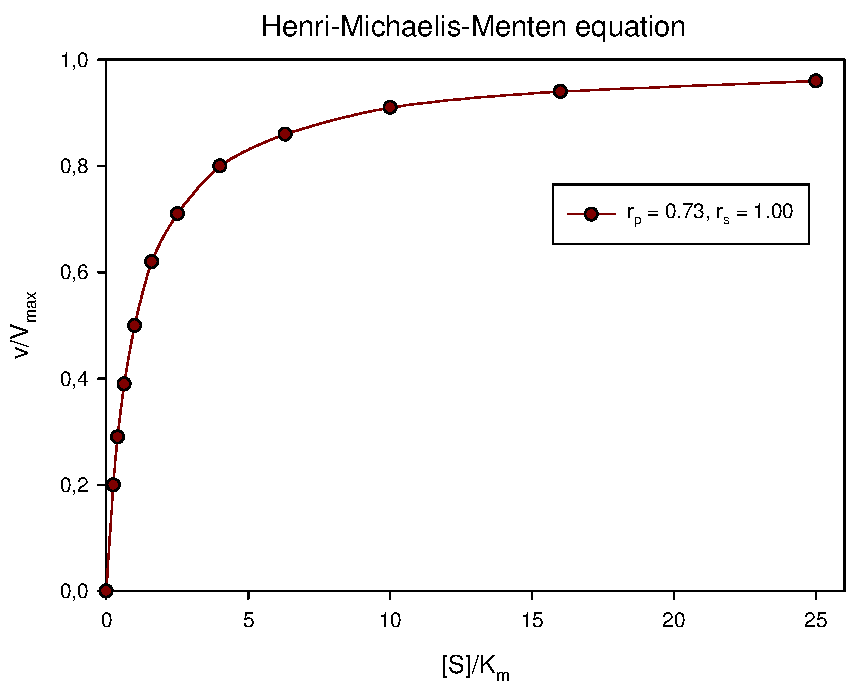
\includegraphics[width=0.75\textwidth]{Graphics/Correlation}
\end{figure}

\skalar{r_s} (\parencite{Spe-04}, often called \textrho) was developed for ordinal scaled variables, however, it can also be used for interval and rational scales. In that case, we work with the rank of each \( \AbsVec{x}_i, \AbsVec{y}_i \) rather than their values. This has the disadvantage of some loss of information, but the advantage that \skalar{r_s} works for non-linear relationships between \AbsVec{x} and \AbsVec{y}, provided only that \AbsVec{y} is a monotonically increasing function of \AbsVec{x} (see fig. \ref{fig:Corr}). For the rank correlation of a linear and a circular variable see chapter \ref{text:circular}.


\begin{lstlisting}[caption=Ranking of a variable]
  PROCEDURE Rank(VAR Data: VectorTyp);

  LABEL
    done;

  VAR
    i, j, k, Valid, n: WORD;
    r, x, y: float;
    Sorted: VectorTyp;

  BEGIN
    n := VectorLength(Data);
    CopyVector(Data, Sorted);
    ShellSort(Sorted);            // create a sorted Copy OF data  (any NaNs TO highest #)
    Valid := n;
    FOR i := 1 TO n DO
      IF IsNaN(GetVectorElement(Sorted, i))
        THEN DEC(Valid);         // determine number OF non-NaN data points
    i := 1;
    REPEAT
      x := GetVectorElement(Sorted, i);
      IF IsNaN(x)
        THEN
        ELSE
          BEGIN
            j := i;
            REPEAT             // find number OF Elements that are equal TO x
              y := GetVectorElement(Sorted, Succ(j));
              IF IsNaN(y)
                THEN GOTO Done // leave counting LOOP, no more valid data
                ELSE IF (x = y)
                       THEN INC(j);
            UNTIL ((x < y) OR (j = n));
  Done:     r := (1.0 * i + j) / 2;     // rank IS average OF lowest + highest element
            FOR k := 1 TO Valid DO      // change all elements OF Data equal TO x -> rank
              BEGIN
                y := GetVectorElement(Data, k);
                IF IsNaN(y)
                  THEN
                  ELSE IF (y = x)
                         THEN SetVectorElement(Data, k, r);
              END;
            i := Succ(j);
          END;
    UNTIL (i >= Valid) OR IsNaN(x);
    DestroyVector(Sorted);
  END;
\end{lstlisting}

The distribution of \skalar{r_s} does not depend on the distribution of \AbsVec{x,y}, so the tests described for \skalar{r_p} can always be used (\skalar{r_s} is non-parametric). The calculation of \skalar{r_s} is performed exactly as described for \skalar{r_p}.

If there are no ties (all x-values different from each other and all y-values different from each other), then there is a computationally simpler form to calculate \skalar{r_s}:
\begin{equation}
  r_s = 1 - \frac{6 \sum_{i=1}^n{(\AbsVec{x}_i - \AbsVec{y}_i)^2}}{n^3-n}
\end{equation}
\skalar{r_s} has no PRE interpretation \parencite{Fre-86}.

\begin{lstlisting}[caption=\Name{Spearman}'s rank correlation coefficient]
  FUNCTION SpearmanRankCorrelation(CONST Vector1, Vector2: VectorTyp;
    VAR Significance: SignificanceType): float;

  VAR
    Ranked1, Ranked2: VectorTyp;

  BEGIN
    IF NOT (TestDataVectorLength(Vector1, Vector2)) THEN EXIT;
    CopyVector(Vector1, Ranked1);
    CopyVector(Vector2, Ranked2);
    Rank(Ranked1);
    Rank(Ranked2);
    Result := PearsonProductMomentCorrelation(Ranked1,
      Ranked2, Significance);
    DestroyVector(Ranked1);
    DestroyVector(Ranked2);
  END;
\end{lstlisting}

\subsubsection{Significance testing of \skalar{r_s}}

A non-zero \skalar{r_s} can be tested for significance by
\begin{equation}
  t = r_s \times \sqrt{\frac{n-2}{1-r_s^2}}
\end{equation}
with \(n-2 \) degrees of freedom.

\subsection{Quadrant correlation \skalar{r_q}}\label{text:quadrant}

The quadrant correlation is measure of correlation robust against outliers. It is calculated from the number of observations in the four quadrants determined by the median pair. The number of observations in quadrant I and III (\skalar{n_+}) and in quadrants II and IV (\skalar{n_-}) are determined:
\begin{equation}
  r_q = \frac{n_+ - n_-}{n_+ + n_-}  = \frac{1}{N} \times \sum_{i=1}^n{\sgn{(\AbsVec{x}_i - \tilde{x})} \times \sgn{(\AbsVec{y}_i - \tilde{y})}}
\end{equation}
with \(\tilde{x},\tilde{y} \) the medians of \AbsVec{X,Y}.

\subsubsection{Median test for significance of \skalar{r_q}}

for the test \(H_0 : r_q = 0 \) \Foreign{vs} \(H_1 : r_q \neq 0 \) calculate (with \(n_e = (n_+ + n_-)/2 \), \(n_e > 5 \)):
\begin{equation}
  \chi^2 \approx \frac{(n_+ - n_e)^2 + (n_- - n_e)^2}{n_e}
\end{equation}
with one degree of freedom.

\begin{lstlisting}[caption=Quadrant correlation and its significance]
  FUNCTION QuadrantCorrelation(CONST Vector1, Vector2: VectorTyp;
    VAR Significance: SignificanceType): float;

  VAR
    Sorted1, Sorted2            : VectorTyp;
    n, i, n_plus, n_minus       : WORD;
    Median1, Median2, x, y, n_e : float;
    c                           : char;

  BEGIN
    IF NOT (TestDataVectorLength(Vector1, Vector2)) THEN EXIT;
    n := VectorLength(Vector1);
    CopyVector(Vector1, Sorted1);
    CopyVector(Vector2, Sorted2);
    Median1 := Median(Sorted1);
    Median2 := Median(Sorted2);
    DestroyVector(Sorted1);
    DestroyVector(Sorted2);
    n_plus := 0;
    n_minus := 0;
    FOR i := 1 TO n DO
      BEGIN
        x := GetVectorElement(Vector1, i);
        y := GetVectorElement(Vector2, i);
        IF IsNaN(x) OR IsNaN(y)
          THEN // ignore NaNs
          ELSE IF ((x = Median1) OR (y = Median2))
                 THEN // ignore data ON coordinate axis OF system WITH origin Median1/Median2
                 ELSE IF (((x > Median1) AND (y > Median2)) OR ((x < Median1) AND (y < Median2)))
                        THEN INC(n_plus)   // concordance: quadrant I OR III
                        ELSE INC(n_minus); // discordance: quadrant II OR IV
      END;
    Result := (n_plus - n_minus) / (n_plus + n_minus);
    n_e := 1.0 * (n_plus + n_minus) / 2;
    IF (n_e < 5)
      THEN
        BEGIN
          c := WriteErrorMessage(' Quadrant correlation: cannot calculate significance because n_e < 5');
          CorrelationsError := TRUE;
          EXIT;
        END;
    Significance.TestValue := ((n_plus - n_e) * (n_plus - n_e) +
      (n_minus - n_e) * (n_minus - n_e)) / n_e;
    Significance.Freedom := 1;
    Significance.P0 := IntegralChi(Significance.TestValue, Round(Significance.Freedom));
  END;
\end{lstlisting}

\section{Binary data}

Association and similarity coefficients for binary data have been reviewed in \parencite{Hub-82}.
Given the confusion table \label{tab:binary}
\begin{tabular}{c|cc}
\toprule
\textsubscript{observed}\textsuperscript{predicted}  & 1 & 0 \\
\midrule
1 & \textcolor{DarkGreen}{TP = a} & \textcolor{DarkRed}{FN = b}   \\
0 & \textcolor{DarkRed}{FP = c}   & \textcolor{DarkGreen}{TN = d} \\
\bottomrule
\end{tabular}\\
the association measure \skalar{r} should meet the following obligatory conditions:
\begin{enumerate}
  \item{For an association measure \(\skalar{r}_{i,j} \leq \skalar{r}_{i,i} \) for all \skalar{i,j} and if \(\skalar{r}_{i,j} > \skalar{r}_{k,l} \) then items \skalar{i,j} are more similar than items \skalar{k,l}.  }
  \item{min(\skalar{r}) should be at \(a = d = 0 \) and max(\skalar{r}) at \(b = c = 0 \).}
  \item{Symmetry: \(\skalar{r}_{i,j} = \skalar{r}_{j,i} \) for all \skalar{i,j}.}
  \item{Discrimination between positive and negative association: \(\skalar{r}(a > a') > \skalar{r}(a<a') \) with \(a' = \frac{(a+b) (a+c)}{n} \).}
  \item{\skalar{r} should be linear with \(\sqrt{\chi^2} \) for both subsets \(ad-bc < 0 \) and \(ad-bc >= 0 \) (note that \(\chi^2 \) violates condition 4).}
\end{enumerate}
and ideally the following non-obligatory conditions:
\begin{enumerate}
  \item[A]{Range of \skalar{r} should be either \(-1\ldots +1 \) or \(0\ldots +1 \). }
  \item[B]{Absolute association: \(\skalar{r}(b=c=0) > \skalar{r}(b = 0 \veebar c = 0) \) (with \(\veebar \) meaning exclusive disjunction (xor)). }
  \item[C]{Nil association at \(a = 0 \): \(\skalar{r}(a=0) = \mathrm{min}(\skalar{r}) \) (stricter than 2) above).}
  \item[D]{Linearity: \(\skalar{r}(a+1) - \skalar{r}(a) = \skalar{r}(a+2) - \skalar{r}(a+1) \). }
  \item[E]{No sensitivity to \(a = 0 \): \(\skalar{r}(a=0,b,c,d), r(a=1,b-1,c-1,d+1), r(a=2,b-2,c-2,d+2)\ldots \) should be smooth}
  \item[F]{Homogeneous distribution of r in permutation samples}
  \item[G]{For random samples from a population with known \skalar{a,b,c,d}, \skalar{r} should show little variability even in small samples.}
  \item[H]{simplicity of calculation, low computer time}
\end{enumerate}
All conditions are met by \Name{Jaccard} \parencite{Jac-08} (\( \frac{a}{a+b+c} = (A \cap B)/(A \cup B) \)), \Name{Russel \& Rao} \parencite{Rus-40} (\( \frac{a}{a+b+c+d} \)) (both range \(0\ldots +1 \)) and \Name{McConnaughey} \parencite{McC-64} (\( \frac{a^2 - bc}{(a+b) (a+c)} \), range \( -1\ldots +1 \)). However, neither of these coefficients has a PRE interpretation.

\begin{lstlisting}[caption=confusion table ]
  FUNCTION ConfusionTable(CONST Vector1, Vector2: VectorTyp): Confusion;

  VAR
    i, n: WORD;      // contingency table values

  BEGIN
    IF NOT (TestDataVectorLength(Vector1, Vector2)) THEN EXIT;
    n := VectorLength(Vector1);
    WITH ConfusionTable DO
      BEGIN
        a := 0;
        b := 0;
        c := 0;
        d := 0;
        FOR i := 1 TO n DO
          IF (IsNaN(GetVectorElement(Vector1, i)) OR IsNaN(GetVectorElement(Vector2, i)))
            THEN // ignore
            ELSE IF (GetVectorElement(Vector1, i) = 1)   // count contingency table elements
                   THEN IF (GetVectorElement(Vector2, i) = 1)
                          THEN INC(a)  // joint presence
                          ELSE INC(b)  // discordance
                   ELSE IF (GetVectorElement(Vector2, i) = 1)
                          THEN INC(c)  // discordance
                          ELSE INC(d); // joint absence
      END;

  END;
\end{lstlisting}

\begin{lstlisting}[caption=\Name{McConnaughey}'s correlation ]
  FUNCTION McConnaugheyCorrelation(c: confusion): float;

  BEGIN
    WITH c DO
      BEGIN
        Result := (1.0 * (a + b) * (a + c));
        IF (Result = 0)
          THEN // shouldn't happen, but result will be 0
          ELSE Result := (1.0 * a * a - 1.0 * b * c) / Result;
      END;
  END;
\end{lstlisting}

\subsection{\Name{Matthews}' correlation \skalar{r_m}}\label{text:Matt}

\Name{Matthews}' correlation \parencite{Mat-75} is used mainly to characterise confusion tables, as it gives balanced results even with very different class sizes:
\begin{equation}
   r_m = \frac{ad - cb}{\sqrt{(a+c) (a+b) (d+c) (d+b)}} = \sqrt{\frac{\chi^2}{n}}
\end{equation}
Should the denominator become zero, \skalar{r_m} is set to zero too, which is the correct limiting value.  In \parencite{Hub-82} \( r_m = A_{30} \) (tetrachoric correlation), its root is called \(A_{31} \) and \( A_{27} = \chi^2 = n r_m^2, 0 \leq r_m \leq \infty \). For clustering, these coefficients are not well suited because
\begin{description}
  \item[\skalar{A_{27}}]{violates conditions 2, 4, D, E}
  \item[\skalar{A_{30}}]{violates conditions C, F }
  \item[\skalar{A_{31}}]{violates conditions 4, D }
\end{description}

\begin{lstlisting}[caption=\Name{Matthews}' correlation ]
  FUNCTION MatthewsCorrelation(c: Confusion): float;

  BEGIN
    WITH c DO
      BEGIN
        Result := 1.0 * (a + c) * (a + b) * (d + c) * (d + b);
        // calculate denominator first
        IF Result <= 0
          THEN // shouldn't happen, but result will be 0, the correct limiting value
          ELSE Result := (a * d - c * b) / Sqrt(Result);
      END;
  END;
\end{lstlisting}

Recall the equation for \Name{Pearson}'s \( r_p = \frac{\cov(x,y)}{\sqrt{\cov(x,x)} \sqrt{\cov(y,y)}} = \frac{\sum_{i=1}^n{(\AbsVec{x}_i - \bar{\AbsVec{x}})(\AbsVec{y}_i - \bar{\AbsVec{y}})}}{\sqrt{(\AbsVec{x}_i - \bar{\AbsVec{x}})^2} \sqrt{(\AbsVec{y}_i - \bar{\AbsVec{y}})^2}}\). The elements of the confusion matrix can be shown to be \( a = \sum_{i=1}^n{\AbsVec{x}_{i}\AbsVec{y}_{i}}, b = \sum_{i=1}^n{\AbsVec{x}_{i}(1-\AbsVec{y}_{i})}, c = \sum_{i=1}^n{(1-\AbsVec{x}_{i})\AbsVec{y}_{i}}, d = \sum_{i=1}^n{(1-\AbsVec{x}_{i})(1-\AbsVec{y}_{i})} \), from which the equation for \skalar{r_m} can be derived. Thus, \skalar{r_m} has \acs{PRE}- and angle-interpretation.

\skalar{r_m} has been generalised to \( k \times k \) confusion matrices \parencite{Gor-04}, for which we use the nomenclature of contingency tables in fig. \ref{ContDef} on page \pageref{ContDef}:
\begin{equation}
  r_k = \frac{\trace(\arr{T}) \times n - \sum_{i=1}^k{(\AbsVec{c}_{i} \AbsVec{r}_{i})}}{\sqrt{(n^2 - \sum_{i=1}^k{\AbsVec{c}_{i}^2}) (n^2 - \sum_{i=1}^k{\AbsVec{r}_{i}^2}) }}
\end{equation}
where \(\trace(\arr{T}) \) (sum of diagonal elements) is the number of correct predictions, the row-sums \( \AbsVec{r}_{i} \) give the number of times that class \skalar{i} occured, the column sums \( \AbsVec{c}_{i} \) the number of times that class \skalar{i} was predicted and \skalar{n} is the total number of observations. The problem with \skalar{r_k} compared to \skalar{r_m} is that although the maximum value remains \(+1\), the minimal value is somewhere between \(-1\) and \num{0}.

\begin{lstlisting}[caption=\Name{Gorodkin}'s multi-class correlation \skalar{r_k}]
  FUNCTION Rk(Cont: ContTable): float;

  VAR
    k, i                   : WORD;
    Sum1, Sum2, Sum3, Sum4 : float;
    c                      : char;

  BEGIN
    k := Cont^.r;
    IF k <> Cont^.c
      THEN
        BEGIN
          c := WriteErrorMessage('Gorodkin''s Rk: Contingency table not square ');
          CorrelationsError := TRUE;
          EXIT;
        END;
    Sum1 := 0;
    Sum2 := 0;
    Sum3 := 0;
    Sum4 := 0;
    FOR i := 1 TO k DO
      BEGIN
        Sum1 := Sum1 + (Cont^.RowSums[i] * Cont^.ColumnSums[i]);
        Sum2 := Sum2 + (Cont^.ColumnSums[i] * Cont^.ColumnSums[i]);
        Sum3 := Sum3 + (Cont^.RowSums[i] * Cont^.RowSums[i]);
        Sum4 := Sum4 + Cont^.Table[i, i];
      END;
    Result := (Sum4 * Cont^.n - Sum1) / Sqrt((Cont^.n * Cont^.n - Sum2) *
      (Cont^.n * Cont^.n - Sum3));
  END;
\end{lstlisting}

In principle, a correlation can be calculated even if the number of classes in the observation \skalar{k} is not equal to the number of classes in the prediction \skalar{l}, resulting in a non-square confusion matrix \( \arr{C}_{k\times l},\quad l \neq k \). In such a confusion matrix, \( \AbsVec{c}_{ij} \) would be the number of elements of observed class \( i \in 1\ldots k\) and predicted class \( j \in 1\ldots l\).

We can then calculate TP, TN, FP and FN for the \skalar{i}-th row (or column), from the number of samples where \skalar{i} is\\
\begin{tabular}{|l|cc|}
  \toprule
                      & observed class & predicted class \\
  \midrule
  TP\textsubscript{i} (=a) & \textcolor{DarkGreen}{\(\checkmark\)} & \textcolor{DarkGreen}{\(\checkmark\)} \\
  FP\textsubscript{i} (=c) & \textcolor{DarkRed}{\(\times\)}       & \textcolor{DarkGreen}{\(\checkmark\)} \\
  TN\textsubscript{i} (=d) & \textcolor{DarkRed}{\(\times\)}       & \textcolor{DarkRed}{\(\times\)}       \\
  FN\textsubscript{i} (=b) & \textcolor{DarkGreen}{\(\checkmark\)} & \textcolor{DarkRed}{\(\times\)}       \\
  \bottomrule
\end{tabular}\\
these are then used to calculate the row- (or column)-wise \skalar{r_i}.

\subsection{\Name{Goodman \& Kruskal}'s \textlambda\ for binary/binary association}

Binary data can be viewed as a special case of nominal, with only two classes. Therefore, the symmetrical version \textlambda\ \parencite{Goo-54} (see below) can be used also for binary/binary associations. \textlambda\ has a PRE interpretation.

\subsection{The point biserial correlation \skalar{r_j} for binary/cardinal association}

\skalar{r_j} is simply the product moment correlation between the rational data and binary data taken as numerical values (usually 0 and 1). As such, \skalar{r_j} has both PRE and angle interpretation \parencite{Cos-65}. There is, however, a numerically more elegant way to calculate it:
\begin{equation}
  r_j = \frac{\bar{X}_1 - \bar{X}_0}{s} \sqrt{\frac{n_1 n_o}{N^2}}
\end{equation}
with \skalar{n_1, n_0} the number of cases who got 1 and 0, respectively, \(N = n_0 + n_1 \) the total number of cases, \skalar{\bar{X}_1, \bar{X}_0} the group averages of cases who got 1 and 0, \(\bar X \) the overall average and with
\begin{equation}
  s = \sqrt{\frac{1}{N} \sum\limits_{i=1}^N (X_i - \bar{X})^2}
\end{equation}
the standard deviation of the total average \skalar{\bar X}.

\skalar{r_j} is used in test theory of binary exams to calculate how well student's results on a particular question mirror their overall performance in the test. When used for this purpose, \skalar{s} needs to be calculated without the question under test, at least if the number of questions is small.

\paragraph{Significance of \skalar{r_{j}}}

A t-test can be used to test \(H_0: r_j = 0 \) \Foreign{vs} \(H_1: r_j \neq 0 \)
\begin{equation}
  t \approx r_j \sqrt{\frac{N-2}{1-r_j^2}}, \quad f = N - 2
\end{equation}

\begin{lstlisting}[caption=PointBiserial correlation and its significance]
  FUNCTION PointBiserialCorrelation(CONST BinaryVector, CardinalVector: VectorTyp;
    VAR Significance: SignificanceType): float;

  VAR
    n, i, TotalI, GoodI, BadI                 : WORD;
    SumX, SumXGood, SumXBad, s, barX, x, y, r : float;
    c                                         : CHAR;

  BEGIN
    IF NOT (TestDataVectorLength(BinaryVector, CardinalVector)) THEN EXIT;
    n := VectorLength(CardinalVector);
    TotalI := 0;
    SumX := 0;
    FOR i := 1 TO n DO       // calculate average x
      IF NOT (IsNaN(GetVectorElement(CardinalVector, i)) OR
              IsNaN(GetVectorElement(BinaryVector, i)))
        THEN
          BEGIN
            INC(TotalI);
            SumX := SumX + GetVectorElement(CardinalVector, i);
          END;
    BarX := SumX / TotalI;
    SumX := 0;
    FOR i := 1 TO n DO       // calculate standard deviation OF x
      IF NOT (IsNaN(GetVectorElement(CardinalVector, i)) OR
              IsNaN(GetVectorElement(BinaryVector, i)))
        THEN
          SumX := SumX + (GetVectorElement(CardinalVector, i) - barX) *
                 (GetVectorElement(CardinalVector, i) - barX);
    s := Sqrt(SumX / TotalI);
    GoodI := 0;
    BadI := 0;
    SumXGood := 0;
    SumXBad := 0;
    FOR i := 1 TO n DO
      IF (IsNaN(GetVectorElement(CardinalVector, i)) OR
          IsNaN(GetVectorElement(BinaryVector, i)))
        THEN  // ignore
        ELSE IF (GetVectorElement(BinaryVector, i) = 1)
               THEN
                 BEGIN
                   INC(GoodI);
                   SumXGood := SumXGood + GetVectorElement(CardinalVector, i);
                 END
               ELSE IF (GetVectorElement(BinaryVector, i) = 0)
                      THEN
                        BEGIN
                          INC(BadI);
                          SumXBad := SumXBad + GetVectorElement(CardinalVector, i);
                        END
                      ELSE
                        BEGIN
                          c := WriteErrorMessage('Point biserial correlation: illegal value in exam table');
                          CorrelationsError := TRUE;
                          EXIT;
                        END;
    IF ((GoodI = 0) OR (BadI = 0))
      THEN
        r := 0
      ELSE
        BEGIN
          SumXGood := SumXGood / GoodI;
          SumXBad := SumXBad / BadI;
          x := Sqrt(GoodI * BadI / TotalI / TotalI);
          y := (SumXGood - SumXBad) / s;
          r := x * y;
        END;
    CorrelationSignificance(BinaryVector, CardinalVector, r, Significance);
    Result := r;
  END;
\end{lstlisting}

\section{Ordinal data}

\begin{table}
  \caption{Contingency table \arr{T} for nominal and ordinal data vectors \AbsVec{X,Y} of length \skalar{n} with definitions of the symbols used in the text. \AbsVec{R,C} are the row- and column-sums, respectively.}
  \label{ContDef}
  \centering
    \begin{tabular}{|c|ccccc|c|}
      \toprule
      \AbsVec{X\backslash Y} & \(\AbsVec{y}_1 \)  & \(\ldots \)  & \(\AbsVec{y}_j \)  & \(\ldots \) & \(\AbsVec{y}_c \) & \AbsVec{R}             \\
      \midrule
 \(\AbsVec{x}_1 \)         & \(\AbsVec{t}_{11} \)  &           &                 &          &                & \(\AbsVec{r}_{1\cdot} \)  \\
 \(\vdots \)               &                 &           &                 &          &                &                        \\
 \(\AbsVec{x}_i \)         &                 &           & \(\AbsVec{t}_{ij} \)  &          &                & \(\AbsVec{r}_{i\cdot} \)  \\
 \(\vdots \)               &                 &           &                 &          &                &                        \\
 \(\AbsVec{x}_r \)         &                 &           &                 &          & \(\AbsVec{t}_{rc} \) & \(\AbsVec{r}_{r\cdot} \)  \\
      \midrule
      \AbsVec{C}             & \(\AbsVec{c}_{\cdot 1} \) & \(\ldots \) & \(\AbsVec{c}_{\cdot j} \) & \(\ldots \) & \(\AbsVec{c}_{\cdot c} \) & \skalar{n} \\
      \bottomrule
    \end{tabular}
\end{table}

Ordinal and nominal data are conveniently summarised in contingency tables like tab. \ref{ContDef}, with \(\AbsVec{t}_{ij} \) the number of data where \(\AbsVec{x} = i \) and \(\AbsVec{y} = j \). \AbsVec{X} is the independent variable and defines the rows of the table, \AbsVec{Y} is the dependent variable and defines the columns. \skalar{n} is the length of the data vectors, \AbsVec{r,c} the number of rows and columns of the contingency table, which is also the number of unique values in \AbsVec{X,Y}, respectively. Conventionally, loop counters are \skalar{i} for rows and \skalar{j} for columns.

\begin{lstlisting}[caption=Handling of contingency tables]
  PROCEDURE Contingency(Data1, Data2: VectorTyp; VAR Cont: ContTable);

  VAR
    i, j, l, m, Length : WORD;
    c                  : char;

  BEGIN
    IF NOT (TestDataVectorLength(Data1, Data2)) THEN EXIT;
    Length := VectorLength(Data1);
    TRY
      GetMem(Cont, SizeOf(ContStruc));
    except
      c := WriteErrorMessage(' Contingency table: Not enough memory to create table');
      EXIT;
    END;
    FOR i := 0 TO MaxSteps DO
      // we don't know number of different values yet, so use maximum
      BEGIN
        FOR j := 0 to MaxSteps DO
          Cont^.Table[i, j] := 0;
        Cont^.RowSums[i] := 0;
        Cont^.ColumnSums[i] := 0;
      END;
    Cont^.n := 0;
    Cont^.r := 0;
    Cont^.c := 0;
    FOR i := 1 TO Length DO
      BEGIN
        IF (IsNaN(GetVectorElement(Data1, i)) OR IsNaN(GetVectorElement(Data2, i)))
          THEN  // ignore
          ELSE
            BEGIN
              l := trunc(GetVectorElement(Data1, i));
              m := trunc(GetVectorElement(Data2, i));
              Inc(Cont^.Table[l, m]);
              IF (l > Cont^.r)
                THEN Cont^.r := l; // set r to highest value of Data1
              IF (m > Cont^.c)
                THEN Cont^.c := m; // set c to highest value of Data2
              Inc(Cont^.n);
            END;
      END;
    FOR i := 0 TO Cont^.r DO
      FOR j := 0 TO Cont^.c DO
        BEGIN
          Cont^.RowSums[i] := Cont^.RowSums[i] + Cont^.Table[i, j];
          Cont^.ColumnSums[j] := Cont^.ColumnSums[j] + Cont^.Table[i, j];
        END;
  END;


  PROCEDURE DestroyContingency(var Cont : ContTable);

  BEGIN
    FreeMem(Cont, SizeOf(ContStruc));
  END;


  PROCEDURE WriteContingency(CONST Cont : ContTable; MedStr : String; ValidFigures : byte);

  VAR i, j    : WORD;
      Medium  : TEXT;
      c       : CHAR;

  BEGIN
    IF (MedStr = 'CON')
      THEN
        BEGIN
          FOR i := 0 TO Cont^.r DO
            BEGIN
              FOR j := 0 TO Cont^.c Do
                write(Cont^.Table[i,j]:ValidFigures, ' ');
              writeln('| ', Cont^.RowSums[i]:ValidFigures);
            END;
          FOR j := 0 TO Cont^.c DO
            FOR i := 1 TO succ(ValidFigures) DO write('_');
          write('|');
          FOR i := 1 TO succ(ValidFigures) DO write('_');
          writeln;
          FOR j := 0 TO Cont^.c DO write(Cont^.ColumnSums[j]:ValidFigures, ' ');
          writeln('| ', Cont^.n:ValidFigures);
        END
      ELSE
        BEGIN
          TRY
            assign(Medium, MedStr);
            rewrite(Medium);
          EXCEPT
            c := WriteErrorMessage(' Writing contingency table: could not open file ', MedStr:length(MedStr));
            CorrelationsError := true;
            EXIT;
          END;
          FOR i := 0 TO Cont^.r DO
            BEGIN
              FOR j := 0 TO Cont^.c DO
                write(Medium, Cont^.Table[i,j]:ValidFigures, ' ');
              writeln(Medium, '| ', Cont^.RowSums[i]:ValidFigures);
            END;
          FOR j := 0 TO Cont^.c DO
            FOR i := 1 TO succ(ValidFigures) DO write(Medium, '_');
          write(Medium, '|');
          FOR i := 1 TO succ(ValidFigures) DO write(Medium, '_');
          writeln(Medium);
          FOR j := 0 TO Cont^.c DO write(Medium, Cont^.ColumnSums[j]:ValidFigures, ' ');
          writeln(Medium, '| ', Cont^.n:ValidFigures);
        END;
  END;
\end{lstlisting}

\subsection{Ordinal/ordinal associations}

According to \parencite{Fre-86}, data on an at least ordinal (but possibly higher) scale can be arranged in an ordered contingency table so that \(\AbsVec{x}_1 < \AbsVec{x}_2 < \ldots < \AbsVec{x}_n \) and \(\AbsVec{y}_1 < \AbsVec{y}_2 < \ldots < \AbsVec{y}_n \). If there are \skalar{n} observations, then there are \(P = {n \choose 2} = (n^2 - n)/2 \) pairs of observation, of which there are\\
\begin{tabular}{ll}
 \(C \)   & concordant pairs \\
 \(D \)   & discordant pairs \\
 \(X_0 \) & pairs tied in only \AbsVec{x} \\
 \(Y_0 \) & pairs tied in only \AbsVec{y} \\
 \(Z \)   & pairs tied in both \AbsVec{x} and \AbsVec{y}
\end{tabular}\\
with \(P = C + D + X_0 + Y_0 + Z \). If \(P = C \), then the data have perfect positive association. Likewise, if \(P = D \), association is perfect but negative. The difference \(C - D \) indicates how much the data follow either of these limiting cases. If \(C = D \) then \AbsVec{x} and \AbsVec{y} are independent and the difference is 0. If instead of absolute numbers the probabilities \(P(C) \) and \(P(D) \) are used, the measure becomes independent of sample size.

Monotonic functions in mathematics can be divided as follows:\\
\begin{tabular}{ll}
  increasing     & for all \(\AbsVec{x}_i > \AbsVec{x}_j \Rightarrow \AbsVec{y}_i > \AbsVec{y}_j, \AbsVec{x}_i = \AbsVec{x}_j \Rightarrow \AbsVec{y}_i = \AbsVec{y}_j \) \\
  decreasing     & for all \(\AbsVec{x}_i > \AbsVec{x}_j \Rightarrow \AbsVec{y}_i < \AbsVec{y}_j, \AbsVec{x}_i = \AbsVec{x}_j \Rightarrow \AbsVec{y}_i = \AbsVec{y}_j \) \\
  non-decreasing & for all \(\AbsVec{x}_i > \AbsVec{x}_j \Rightarrow \AbsVec{y}_i \geq \AbsVec{y}_j \) \\
  non-increasing & for all \(\AbsVec{x}_i > \AbsVec{x}_j \Rightarrow \AbsVec{y}_i \leq \AbsVec{y}_j \) \\
\end{tabular}\\
In statistics, however, several repetitions of measurements for a \(\AbsVec{x}_i \) may (and usually will) result in different \AbsVec{y}-values, due to measurement error. We are therefore not dealing with \emph{functions}, but with \emph{relations}. \(Z \)-ties occur if all measurements of \(\AbsVec{x}_i \) result in the same \(\AbsVec{y}_i \), they are \emph{replications} that occur in the same cell of the contingency table and have no effect on the model. When mapping from \AbsVec{X} to \AbsVec{Y}, monotonic one-to-one relations disallow both \(X_0 \)-ties and \(Y_0 \)-ties, monotonic functions (many to one) exclude \(X_0 \)-ties, but \(Y_0 \)-ties are allowed. In monotonic relations (many to many), both are allowed. These three models have different association measures, with different PRE interpretation:

\subsubsection{\Name{Kendall}'s \(\tau \) for monotonic relations with \(X_0 = Y_0 = Z = 0 \)}

If we guess the order of \AbsVec{Y} without reference to \AbsVec{x}, then \(\AbsVec{y}_i > \AbsVec{y}_j \) has a probability of 1/2 and \(E_1 = (C+D)/2 \). If we take \AbsVec{X} into account, we guess concordance for all pairs if \(C>D \) and discordance if \(D>C \). Then \skalar{E_2} is the smaller of \skalar{C} and \skalar{D} and
\begin{equation}
  \tau = \frac{(C+D)/2 - D}{(C+D)/2} = \frac{C-D}{C+D}
\end{equation}
For an example, see table \ref{tab:ExampleGamma}.

\begin{table}
  \caption{Example data for the calculation of \(\tau \) and \(\gamma \), taken from \parencite{Fre-65}, p. 84}
  \label{tab:ExampleGamma}
  \centering
    \begin{tabular}{lrrrr}
      \toprule
      Family interest & Expert Rank & Empirical Rank & Inversion (D) & Agreement (C) \\
      \midrule
      Demonstrating affection & 10 &  9 &  0 &  0 \\
      Planning for future     &  9 &  6 &  0 &  1 \\
      Planning saving         &  8 & 10 &  2 &  0 \\
      Training children       &  7 &  1 &  0 &  3 \\
      Planning budget         &  6 &  8 &  2 &  2 \\
      Plans for children      &  5 &  7 &  2 &  3 \\
      Home decoration         &  4 &  4 &  1 &  5 \\
      Preparing meals         &  3 &  5 &  2 &  5 \\
      Shopping                &  2 &  3 &  1 &  7 \\
      Housecleaning           &  1 &  2 &  1 &  8 \\
      \midrule
      Totals                  &    &    & 11 & 34 \\
      \bottomrule
    \end{tabular}
    \begin{equation}
      \gamma = \frac{C-D}{C+D} = \frac{34-11}{34+11} = 0.511
    \end{equation}
\end{table}

\subsubsection{\Name{Goodman \& Kruskal}'s \skalar{\gamma} if ties are ignored}

The same reasoning applies as for \skalar{\tau}, except that ties are not prohibited, but simply ignored.

\subsubsection{\Name{Kim}'s \skalar{d_{y.x}} for monotonic functions}

We choose only data pairs where \(y_i \neq y_j \), and therefore eliminate \(Y_0 \) and \(Z \). Then the initial guessing error is 1/2 for all remaining pairs, that is, \(E_1 = 1/2 (C+D+X_0) \). If we guess taking \AbsVec{X} into account as discussed above, the cases where \(\AbsVec{x}_i = \AbsVec{x}_j \) give us no information and their error is 1/2. This has to be added to the errors for the untied cases and \(E_2 = D + X_0/2 \)
\begin{align}
  d_{y.x} &= \frac{C-D}{C+D+X_0} \\
  d_{x.y} &= \frac{C-D}{C+D+Y_0}
\end{align}
\skalar{d_{y.x}} (dependent \AbsVec{Y} from independent \AbsVec{X}) and \skalar{d_{x.y}} (dependent \AbsVec{X} from independent \AbsVec{Y}) are asymmetric measures of association, which have PRE interpretation. The average of \(d_{x.y} \) and \(d_{y.x} \), however, cannot be used as a symmetric PRE measure of association.

\subsubsection{\Name{Wilson}'s \skalar{e} for monotonic one-to-one correspondence}

The guessing to determine \skalar{E_1} and \skalar{E_2} are performed twice, for \AbsVec{X} and \AbsVec{Y}. To guess \AbsVec{Y}, we make the condition that \(\AbsVec{x}_i \neq \AbsVec{x}_j \), and to guess \AbsVec{X}, we make the condition that \(\AbsVec{y}_i \neq \AbsVec{y}_j \).
\begin{align}
   E_1(Y) &= (C+D)/2 + Y_0 \\
   E_1(X) &= (C+D)/2 + X_0 \\
   E_1    &= E_1(X) + E_1(Y) = C+D+X_0-Y_0\\
   E_2(Y) &= D + Y_0 \\
   E_2(X) &= D + X_0 \\
   E_2    &= E_2(X) + E_2(y) = 2D + X_0 + Y_0 \\
   e      &= \frac{C-D}{C+D+X_0+Y_0}
\end{align}
is a symmetrical measure of association with PRE interpretation. In the special case of \(X_0=Y_0=Z=0 \) then \(\tau = e \).

\subsubsection{Significance testing of these coefficients}

For \(n > 10 \), the limiting sampling distribution of \(S = |C-D| \) is the normal distribution, even when ties are present. If there is no correlation between \AbsVec{X} and \AbsVec{Y} then \(E(\gamma) = 0 \). \skalar{S} should be corrected for the step-wise (rather than smooth) distribution according to
\begin{equation}
  \hat{S} = |C-D| - \frac{n}{2 (R-1) (C-1)}
\end{equation}
and the standard error of \(\hat{S} \) is
\begin{equation}
  s = \sqrt{\frac{U_2V_2}{n-1} - \frac{U_2V_3 + V_2U_3}{n (n-1)} + \frac{U_3V_3}{n (n-1) (n-2)}}
\end{equation}
with \(U_x, V_x \) the sum of products of row and column totals taken x at a time. Example (taken from \parencite{Fre-65}):

\begin{tabular}{r|rrrr|r}
  \toprule
  y \( \backslash \) x & 4 & 3 & 2 & 1 & \skalar{r} \\
  \midrule
  2              & 4 & 5 & 0 & 1 & 10 \\
  1              & 0 & 2 & 6 & 4 & 12 \\
  \midrule
  \AbsVec{C}     & 4 & 7 & 6 & 5 & 22 \\
  \bottomrule
\end{tabular}

Then
\begin{align*}
  U_2 &= 10 \times 12 = 120 \\
  V_2 &= 4 \times 7 + 4 \times 6 + 4 \times 5 + 7 \times 6 + 7 \times 5 + 6 \times 5 = 179 \\
  U_3 &= 0 \qquad \mathrm{since\ there\ are\ only\ two\ rows} \\
  V_3 &= 4 \times 7 \times 6 + 4 \times 7 \times 5 + 4 \times 6 \times 5 = 638 \\
  s   &= \sqrt{\frac{120 \times 179}{21} - \frac{120 \times 638 + 179 \times 0}{22 \times 21} + \frac{0}{22 \times 21 \times 20}} \\
      &= \sqrt{1022.86 - 165.07 + 0} = \sqrt{857.79} = 29.29 \\
  \hat{S} &= |98 - 8| - \frac{22}{2  \times 1 \times 3} = 90 - 3.67 = 86.33 \\
  z &= \frac{\hat{S}}{s} = \frac{86.33}{29.29} = 2.95
\end{align*}
\skalar{z} is so large that the probability of the Null-hypothesis is less than \num{0.01}.

\begin{lstlisting}[caption= Correlation coefficients for ordinal/ordinal associations]
  FUNCTION OrdinalCorrelations(CONST Data1, Data2: VectorTyp; Formula: CHAR;
    VAR Significance: SignificanceType): float;

  VAR
    i, j, k, C, D, X0, Y0, Z, Length: WORD;
    x1, x2, y1, y2, U2, U3, V2, V3: float;
    Cont: ContTable;

  BEGIN
    IF NOT (TestDataVectorLength(Data1, Data2)) THEN EXIT;
    Length := VectorLength(Data1);
    Contingency(Data1, Data2, Cont);
    C := 0;
    D := 0;
    X0 := 0;
    Y0 := 0;
    Z := 0;
    FOR i := 1 TO Length DO
      FOR j := Succ(i) TO Length DO
        BEGIN
          x1 := GetVectorElement(Data1, i);
          x2 := GetVectorElement(Data1, j);
          y1 := GetVectorElement(Data2, i);
          y2 := GetVectorElement(Data2, j);
          IF (IsNaN(x1) OR IsNaN(x2) OR IsNaN(y1) OR IsNaN(y2))
            THEN // ignore NaNs
            ELSE IF (Trunc(x1) = Trunc(x2))
                   THEN IF (Trunc(y1) = Trunc(y2))
                          THEN INC(Z)                   // tie IN X AND Y
                          ELSE INC(X0)                  // tie IN X only
                   ELSE IF (Trunc(y1) = Trunc(y2))
                          THEN INC(Y0)                  // tie IN Y only
                          ELSE IF (Trunc(x1) > Trunc(x2))
                                THEN IF (Trunc(y1) > Trunc(y2))
                                    THEN INC(C)
                                    ELSE INC(D)
                                ELSE IF (Trunc(y1) > Trunc(y2))
                                       THEN INC(D)
                                       ELSE INC(C);
        END; // FOR j
    CASE UpCase(Formula) OF
      'T', 'G': BEGIN  // calculate Kendal's tau or Goodman & Kruskal's gamma
                  Result := (1.0 * C + D);
                  IF (Result = 0)
                    THEN      // ???
                    ELSE Result := (1.0 * C - D) / Result;
                END;
      'D':      BEGIN  // calculate Kim's d_{xy} (note that d_{xy} <> d_{yx})
                  Result := C + D + X0;
                  if (Result = 0)
                    then      // ???
                    else Result := (1.0 * C - D) / Result;
                end;
      'E':      begin  // calculate Wilson's e
                  Result := C + D + X0 + Y0;
                  IF (Result = 0)
                    THEN      // ???
                    ELSE Result := (1.0 * C - D) / Result;
                END;
    END; // case
    U2 := 0; // now start WITH significance
    FOR i := 0 TO Cont^.r DO
      FOR j := Succ(i) TO Cont^.r DO
        U2 := U2 + Cont^.RowSums[i] * Cont^.RowSums[j];
    // sum OF product OF row sums 2 at a time
    V2 := 0;
    FOR i := 0 TO Cont^.c DO
      FOR j := Succ(i) TO Cont^.c DO
        U2 := U2 + Cont^.ColumnSums[i] * Cont^.ColumnSums[j];
    // sum OF product OF column sums 2 at a time
    U3 := 0;
    FOR i := 0 TO Cont^.c DO
      FOR j := Succ(i) TO Cont^.c DO
        FOR k := Succ(j) TO Cont^.c DO
          U3 := U3 + Cont^.RowSums[i] * Cont^.RowSums[j] * Cont^.RowSums[k];
    // sum OF product OF row sums 3 at a time
    V3 := 0;
    FOR i := 0 TO Cont^.c DO
      FOR j := Succ(i) TO Cont^.c DO
        FOR k := Succ(j) TO Cont^.c DO
          U3 := U3 + Cont^.ColumnSums[i] * Cont^.ColumnSums[j] * Cont^.ColumnSums[k];
    // sum of product of column sums 3 at a time
    Significance.Freedom := Sqrt(U2 * V2 / Pred(Cont^.n) - (U2 * V3 + V2 * U3) /
      (Cont^.n * Pred(Cont^.n)) + U3 * V3 / (Cont^.n * Pred(Cont^.n) * (Cont^.n - 2)));
    // standard deviation
    Significance.P0 := 0;
    // if it can't be calculated
    Significance.TestValue := (2 * pred(Cont^.r) * pred(Cont^.c));
    IF (Significance.TestValue <> 0) THEN
      Significance.TestValue := abs(C - D) - Cont^.n / Significance.TestValue; // average
    IF (Significance.Freedom <> 0) THEN
      Significance.P0 := IntegralGauss(Significance.TestValue / Significance.Freedom);
    // error corresponding to z
  END;
\end{lstlisting}

\section{Nominal data}

\subsection{Intraclass correlation for nominal/cardinal association}

\begin{figure}
   \caption{High intraclass correlation: each class (\AbsVec{x}) is associated with a particular range of \AbsVec{y}-values. Note that since \AbsVec{x} is on a nominal scale the order of \AbsVec{x}-values is random. The rank correlation coefficient \(\skalar{r_s} = 0.04 \), but \(\skalar{r_i} = 0.94 \). }
   \label{fig:Interclass}
   \centering
      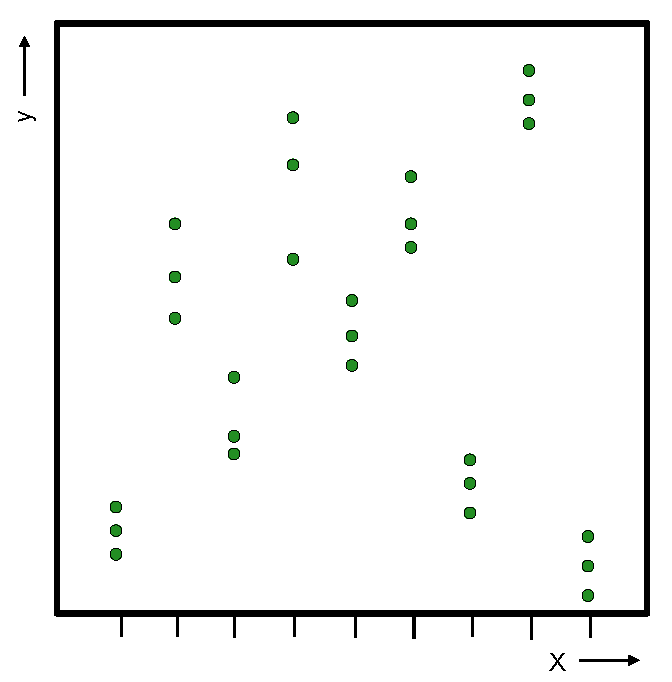
\includegraphics[width=0.75\textwidth]{Graphics/Intraclass}
\end{figure}

For nominally scaled data, neither \skalar{r_p} nor \skalar{r_s} is appropriate. However, we can use \skalar{r_i} \parencite{Har-13} to check wether certain values of \AbsVec{y} concentrate in certain classes of \AbsVec{x} (see fig. \ref{fig:Interclass}). If we have \skalar{A} groups with \skalar{B} data points per group, then \skalar{r_i} becomes:
\begin{align}
  r_i & = \frac{B}{B-1} \frac{A^{-1} \sum_{a=1}^A{(\bar{\AbsVec{y}}_a - \bar{\AbsVec{y}})^2}}{s^2} - \frac{1}{B - 1}  \\
      & \approx \frac{A^{-1} \sum_{a=1}^A{(\bar{\AbsVec{y}}_a - \bar{\AbsVec{y}})}}{s^2} \quad \mathrm{for\ large\ } B \\
  s^2 & = \frac{1}{AB} \sum_{b=1}^B{\sum_{a=1}^A{(\AbsVec{y}_{a,b} - \bar{\AbsVec{y}})^2}}
\end{align}
with \(\bar{\AbsVec{y}}_a \) the arithmetic mean of the \AbsVec{y}-values in the \skalar{a}-th group. Biggest limitation of \skalar{r_i} is that all groups need to have the same number of data points, \skalar{B}.

\subsection{\Name{Cramér}'s \skalar{V} for nominal/nominal association}

To compare two nominal scaled data vectors, each of length \skalar{n}, on uses a contingency table \arr{T} with \skalar{r} rows and \skalar{c} columns. Then \skalar{\chi^2} is calculated as follows:
\begin{align}
  \AbsVec{H}_i &= \sum_{j=1}^c{\frac{\arr{T}_{i,j}^2}{\AbsVec{C}_j}} \\
  A      &= \sum_{i=1}^r{\frac{\AbsVec{H}_i}{\skalar{r}_i}} \\
  \chi^2 &= (A-1) \times n \\
  f      &= (r-1) (c-1) \\
\end{align}
with \(\AbsVec{C}_j \) the column sums, \(\skalar{r}_i \) the row sums of the contingency table and \skalar{f} the degrees of freedom \parencite{Pea-00}. With \(\varphi^2 = \chi^2 / n \)
\begin{equation}
  V = \sqrt{\frac{\varphi^2}{\mathrm{min}(r-1, c-1)}}
\end{equation}
\skalar{V} reaches from \(0\ldots 1 \) (\emph{not} \(-1\ldots 1 \), with nominal values increase and decrease have no meaning!),  but tends to overestimate the strength of association between the data vectors. To correct for this bias, \skalar{\tilde{V}} is used:
\begin{align}
  \tilde{V} &= \sqrt{\frac{\tilde{\varphi}^2}{\mathrm{min}(\tilde{r}-1, \tilde{c}-1)}} \\
  \tilde{\varphi}^2 &= \mathrm{max}(0, \varphi^2 - \frac{(c-1)\times (r-1)}{(n-1)}) \\
  \tilde{c} &= c - \frac{(c-1)^2}{(n-1)} \\
  \tilde{r} &= r - \frac{(r-1)^2}{(n-1)}
\end{align}
To test for significance (\( H_0 \): no association between variables) one uses the \( \chi^2 \)-test with \skalar{f} degrees of freedom. \skalar{V} does not have a PRE interpretation.

\begin{lstlisting}[caption=Common correlation measures without PRE-interpretation for enumeration types]
  FUNCTION Chi2(const Contingency: ContTable;
    var Significance: SignificanceType): float;

  VAR
    H: array[0..MaxSteps] of float;
    i, j: word;
    A: float;

  BEGIN
    FOR i := 1 TO MaxSteps DO
      H[i] := 0.0;
    FOR i := 0 TO Contingency^.r DO
      FOR j := 0 TO Contingency^.c DO
        BEGIN
          A := Contingency^.Table[i, j];
          IF Contingency^.ColumnSums[j] = 0
            THEN A := 0
            ELSE A := A * A / Contingency^.ColumnSums[j];
          H[i] := H[i] + A;
        END;
    A := 0;
    FOR i := 0 TO Contingency^.r DO  // calculate first phi^2 = chi^2 / n
      BEGIN
        IF (Contingency^.RowSums[i] = 0)
          THEN
          ELSE A := A + H[i] / Contingency^.RowSums[i];
      END;
    A := (A - 1) * Contingency^.n;
    Significance.TestValue := A;
    Significance.Freedom := pred(Contingency^.r) * pred(Contingency^.c);
    Significance.P0 := IntegralChi(Significance.TestValue, round(Significance.Freedom));
    Result := A;
  END;


  FUNCTION Phi2(CONST Contingency: ContTable;
    VAR Significance: SignificanceType): float;

  VAR
    x: float;

  BEGIN
    x := chi2(Contingency, Significance);
    Result := x / Contingency^.n;
  END;

  FUNCTION CramersVTilde(chi2: float; r, c, n: word): float;

  VAR
    phi2, hilfs, ct, rt: float;

  BEGIN
    phi2 := chi2 / n;
    hilfs := phi2 - pred(c) * pred(r) / pred(n);     // now calculate tilde-version
    IF hilfs > 0
      THEN phi2 := hilfs
      ELSE phi2 := 0;
    ct := c - PRED(c) * PRED(c) / PRED(n);
    rt := r - PRED(r) * PRED(r) / PRED(n);
    IF rt > ct
      THEN rt := ct;                        // determine min(r~,c~)
    Result := sqrt(phi2 / (rt - 1));
  end;
\end{lstlisting}

\subsection{\Name{Guttman}'s coefficient of relative predictability \(\lambda \) for nominal/nominal association}

A different approach to measuring association is to attempt to predict the values of one variable in two different ways \parencite{Gut-41,Gin-06,Goo-54}. First, the values for one variable are predicted without knowing the values of a second variable. Then the values of the first variable are predicted again, after taking into account the values of the second variable. The extent to which the error of prediction for values of one variable can be reduced by knowing the value of a second variable forms the basis for the reduction in error approach to measuring association.

If the variables are cross-tabulated as described for \Name{Cramér}'s \skalar{V} above, then without knowledge of the columns one would pick that row \skalar{i} with the largest row-sum \(\skalar{r}_i \), as this prediction would minimise prediction error, which is \(E_n = n - \skalar{r}_i \).

If, however, it is known that the same individual is in column \skalar{j}, then one would pick the \skalar{i} such that \(\arr{T}_{i,j} \) is maximal, and the prediction error would become \(\AbsVec{C}_j - \arr{T}_{i,j} \). The total prediction error \skalar{E_j} is obtained by summing up the errors thus obtained for all rows.

\skalar{\lambda} is defined as the proportional reduction in error (PRE), that is
\begin{equation}
  \lambda = \frac{E_n - E_j}{E_n}
\end{equation}
and is the fraction by which the prediction error for the dependent variable can be reduced by knowledge of independent. For example, \(\lambda = 0.63 \) means that the error can be reduced by \SI{63}{\%} or about 2/3. Therefore, \(0 \leq \lambda \leq 1 \), with \(\lambda = 0 \) meaning no association, \(\lambda = 1 \) meaning perfect association. Thus:
\begin{align}
  EC_j &= \AbsVec{C}_j - \mathrm{max}(\arr{T}_{\cdot,j}) \\
  EC   &= \sum_{j=1}^c{EC_j} \\
  ET_r &= n - \mathrm{max}_i(\skalar{r}) \\
  \lambda_r &= \frac{ET_r - E_c}{ET_r} = \frac{n - \mathrm{max}_i(\skalar{r}) - \sum_{j=1}^r{(\AbsVec{C}_j -\mathrm{max}(\arr{T}_{\cdot,j}))}}{n - \mathrm{max}_i(\skalar{r})}
\end{align}
and analogous for \skalar{\lambda_c}:
\begin{align}
  ER_i &= \skalar{r}_i - \mathrm{max}(\arr{T}_{i,\cdot}) \\
  ER   &= \sum_{i=1}^c{EC_i} \\
  ET_c &= n - \mathrm{max}_j(\AbsVec{C}) \\
  \lambda_c &= \frac{ET_c - ER}{ET_c} = \frac{n - \mathrm{max}_j(\AbsVec{C}) - \sum_{i=1}^c{(\skalar{r}_i -\mathrm{max}(\arr{T}_{i,\cdot}))}}{n - \mathrm{max}_j(\AbsVec{C})}
\end{align}
Note that \skalar{\lambda_r} and \skalar{\lambda_c} are usually not identical. \parencite{Goo-54} gives a formula to calculate a symmetrical version of \skalar{\lambda}:
\begin{equation}
  \lambda = \frac{\sum_{i=1}^r{\mathrm{max}(\arr{T}_{i,\cdot})} + \sum_{j=1}^c{\mathrm{max}(\arr{T}_{\cdot,j})} - \mathrm{max}_i(\skalar{r}) - \mathrm{max}_j(\AbsVec{C})}{2n - [\mathrm{max}_i(\skalar{r}) + \mathrm{max}_j(\AbsVec{C})]}
\end{equation}
An almost identical result is obtained by calculating the average of \skalar{\lambda_r} and \skalar{\lambda_c} by eqn. \ref{eqn:AvCorr}.

\begin{table}
  \caption{Example data from \parencite{Goo-54}: Hair colour \Foreign{vs}. eye color. The results for various measures of association are given at the bottom. }
  \label{}
  \centering
    \begin{tabular}{c|cccc|c}
      \toprule
      Eye \(\backslash \) Hair & Fair & Brown & Black & Red  & \skalar{r} \\
      \midrule
      Blue       & 1768 &  807  &  189  &   47 & 2811       \\
      Grey/Green &  946 & 1387  &  746  &   53 & 3132       \\
      Brown      &  115 &  438  &  288  &   16 &  857       \\
      \midrule
      \AbsVec{C} & 2829 & 2632  & 1223  &  116 & n = 6800   \\
      \bottomrule
    \end{tabular}\\
    \vspace{2ex}

    \begin{tabular}{lllll}
 \(\lambda_r \) & \(\lambda_c \) & \(\lambda \) & \(\phi^2 \) & \(V \)    \\
      \midrule
      0.2241      & 0.1924      & 0.2076    & 0.1581   & 0.2812 \\
    \end{tabular}
\end{table}

\begin{lstlisting}[caption=\Name{Guttman}'s asymmetrical and symmetrical \skalar{\lambda}]
  FUNCTION lambda(CONST Contingency: ContTable): float;

  VAR
    i, j: word;
    MaxR, MaxC, SumMaxTi, SumMaxTj: float;
    MaxTi, MaxTj: ARRAY[0..MaxSteps] OF WORD;
    // can't be vectorType AS 0 must be legal index

  BEGIN
    FOR i := 0 TO MaxSteps DO
      BEGIN
        MaxTi[i] := 0;
        MaxTj[i] := 0;
      END;
    SumMaxTi := 0;
    FOR i := 0 TO Contingency^.r DO
      BEGIN
        FOR j := 0 TO Contingency^.c DO
          IF MaxTi[i] < Contingency^.Table[i, j] THEN
            MaxTi[i] := Contingency^.Table[i, j];
        SumMaxTi := SumMaxTi + MaxTi[i];
      END;
    SumMaxTj := 0;
    FOR j := 0 TO Contingency^.c DO
      BEGIN
        FOR i := 0 TO Contingency^.r DO
          IF MaxTj[j] < Contingency^.Table[i, j]
            THEN MaxTj[j] := Contingency^.Table[i, j];
        SumMaxTj := SumMaxTj + MaxTj[j];
      END;
    MaxR := Contingency^.RowSums[0];
    FOR i := 1 TO Contingency^.r DO
      IF (Contingency^.RowSums[i] > MaxR)
        THEN MaxR := Contingency^.RowSums[i];
    MaxC := Contingency^.ColumnSums[0];
    FOR j := 1 TO Contingency^.c DO
      IF (Contingency^.ColumnSums[j] > MaxC)
        THEN MaxC := Contingency^.ColumnSums[j];
    Result := (2 * Contingency^.n - (MaxR + MaxC));
    IF Result = 0
      THEN           // ???
      ELSE lambda := (SumMaxTi + SumMaxTj - MaxR - MaxC) / lambda;
  END;


  FUNCTION lambda_r(CONST Contingency: ContTable): float;

  VAR
    i, j: WORD;
    MaxR, MaxT, SumCT: float;

  BEGIN
    MaxR := 0;
    FOR i := 0 TO Contingency^.r DO
      IF (Contingency^.RowSums[i] > MaxR)
        THEN MaxR := Contingency^.RowSums[i];
    SumCT := 0;
    FOR j := 0 TO Contingency^.c DO
      BEGIN
        MaxT := Contingency^.Table[0, j];
        FOR i := 1 TO Contingency^.r DO
          IF (MaxT < Contingency^.Table[i, j])
            THEN MaxT := Contingency^.Table[i, j];
        SumCT := SumCT + Contingency^.ColumnSums[j] - MaxT;
      END;
    Result := Contingency^.n - MaxR;
    IF (Result = 0)
      THEN          // ???
      ELSE lambda_r := (Contingency^.n - MaxR - SumCT) / lambda_r;
  END;


  FUNCTION lambda_c(CONST Contingency: ContTable): float;

  VAR
    i, j: WORD;
    MaxC, MaxT, SumRT: float;

  BEGIN
    MaxC := 0;
    FOR j := 0 TO Contingency^.c DO
      IF (Contingency^.ColumnSums[j] > MaxC)
        THEN MaxC := Contingency^.ColumnSums[j];
    SumRT := 0;
    FOR i := 0 TO Contingency^.r DO
      BEGIN
        MaxT := Contingency^.Table[i, 0];
        FOR j := 1 TO Contingency^.c DO
          IF (MaxT < Contingency^.Table[i, j])
            THEN MaxT := Contingency^.Table[i, j];
        SumRT := SumRT + Contingency^.RowSums[i] - MaxT;
      END;
    lambda_c := (Contingency^.n - MaxC);
    IF lambda_c = 0
      THEN          // ???
      ELSE lambda_c := (Contingency^.n - MaxC - SumRT) / lambda_c;
  END;
\end{lstlisting}


\subsection{\Name{Freeman}'s measure of association \skalar{\theta} for nominal/ordinal association}

\skalar{\theta}\ measures the reduction of error if an ordinal dependent variable is predicted from an independent variable on the nominal scale, compared to random guessing \parencite{Fre-65,Fre-76}. It is therefore a PRE measure of association. Because variables on the nominal scale are unordered \skalar{\theta} can have only positive values, ranging from \(0\ldots 1 \):
\begin{equation}
  \theta = \frac{\sum_{i=1}^{r}{D_i}}{T}
\end{equation}
with \(D_i = |f_b - f_a| \) for each comparison the difference of frequencies below and above, and \skalar{T} the number of comparisons made. Ties are considered to arise from our inability to precisely rank people and should be split between orders, however, \(|(f_b - 1/2 f_\mathrm{ties}) - (f_a - 1/2 f_\mathrm{ties}) = |f_b - f_a| \), so ties are ignored. \parencite{Fre-65} gives as example social adjustment (ranked, \Foreign{i.e.}, ordinal) \Foreign{vs.} marital status (nominal):

\begin{tabular}{l|rrrrr|r}
  \toprule
  Status \( \backslash \) Rank & 5  & 4  & 3  & 2  & 1  & \(\arr{S} \) \\
  \midrule
  Single   &  1 &  2 &  5 &  2 &  0 & 10 \\
  Married  & 10 &  5 &  5 &  0 &  0 & 20 \\
  Widowed  &  0 &  0 &  2 &  2 &  1 &  5 \\
  Divorced &  0 &  0 &  0 &  2 &  3 &  5 \\
  \bottomrule
\end{tabular}

For the comparison of single and married persons, we get:

\begin{tabular}{r|rrrrr}
  \toprule
  Rank & \(n_r \)  & \(n_b \)  & \(\Pi_b \) & \(n_a \)  & \(\Pi_a \) \\
  \midrule
  5    &     1  &   10   &   10    &    0   &      0  \\
  4    &     2  &    5   &   10    &   10   &     20  \\
  3    &     5  &    0   &    0    &   15   &     75  \\
  2    &     2  &    0   &    0    &   20   &     40  \\
  1    &     0  &    0   &    0    &   18   &      0  \\
  \midrule
 \(f \)  &        &        &   20    &        &    135  \\
  \bottomrule
\end{tabular}

and \(\skalar{D_i} = |f_b - f_a| = |20 - 135| = 115 \). For single and widowed persons, we get:

\begin{tabular}{r|rrrrr}
  \toprule
  Rank & \(n_r \)  & \(n_b \)  & \(\Pi_b \) & \(n_a \)  & \(\Pi_a \) \\
  \midrule
  5    &     1  &    5   &    5    &    0   &      0  \\
  4    &     2  &    5   &   10    &    0   &      0  \\
  3    &     5  &    3   &   15    &    0   &      0  \\
  2    &     2  &    1   &    2    &    2   &      4  \\
  1    &     0  &    0   &    0    &    4   &      0  \\
  \midrule
 \(f \)  &        &        &   32    &        &      4  \\
  \bottomrule
\end{tabular}

and \(\skalar{D_i} = |f_b - f_a| = |32 - 4| = 28 \).  Analogously for the other comparisons:

\begin{tabular}{llrrr}
  \toprule
  Status 1 & Status 2 & \(f_b \) & \(f_a \) & \(D_i \) \\
  \midrule
  single   & divorced &  46   & 0 &  46 \\
  married  & widowed  &  90   & 0 &  90 \\
  married  & divorced & 100   & 0 & 100 \\
  widowed  & divorced &  16   & 2 &  14 \\
  \bottomrule
\end{tabular}

Thus, \(\sum{D_i} = 115 + 28 + 46 + 90 + 100 + 14 = 393 \). \skalar{T} is calculated from the row sums of the data table:
\begin{equation}
  T = 10*20 + 10*5 + 10*5 + 20*5 + 20*5 + 5*5 = 525
\end{equation}
Then \(\theta = 393/525 = 0.75 \)

\subsubsection{Significance of \(\theta \)}

The distribution of \(\theta \) is unknown. If the nominal vector has only two different values, the \Name{Wilcoxon-Mann-Whitney} U-test (first published in \parencite{Deu-14}) can be used.

\begin{lstlisting}[caption=\Name{Freeman}'s measure of association \skalar{\theta}]
  FUNCTION theta(CONST Contingency: ContTable): float;

  VAR
    i, j, k, l: word;
    SumT, fa, fb, SumDi, nr: float;

  BEGIN
    SumT := 0;
    FOR i := 0 TO Contingency^.r DO
      FOR j := succ(i) TO Contingency^.r DO
        SumT := SumT + Contingency^.RowSums[i] * Contingency^.RowSums[j];
    SumDi := 0;
    FOR i := 0 TO Contingency^.r DO
      BEGIN
        FOR k := succ(i) TO Contingency^.r DO
          BEGIN
            fa := 0;
            fb := 0;
            FOR j := 0 TO Contingency^.c DO
              BEGIN
                nr := Contingency^.Table[i, j];
                IF (j < Contingency^.c)
                  THEN
                    FOR l := succ(j) TO Contingency^.c DO
                      fa := fa + Contingency^.Table[k, l] * nr;
                IF (j > 0)
                  THEN // this check actually is necessary
                    FOR l := pred(j) DOWNTO 0 DO
                      fb := fb + Contingency^.Table[k, l] * nr;
              END;
            SumDi := SumDi + abs(fb - fa);
          END;
      END;
    IF (SumT = 0)
      THEN Result := 0    // ???
      ELSE Result := SumDi / SumT;
  END;
\end{lstlisting}


\subsection{\skalar{\eta^2} for nominal/cardinal association}

\skalar{\eta^2} is also a PRE measure \parencite{Ano-16}. Assume we have a vector \AbsVec{y} of cardinal (interval or rational) data. If we had to predict a \(\AbsVec{y}_i \), we would use the arithmetic mean \(\bar{\AbsVec{y}} \) and the prediction error becomes
\begin{equation}
  E_1 = \sum_{i=1}^n{(y_i - \bar{y})^2}
\end{equation}
If, however, we know that the test person \skalar{i} belongs into group \skalar{k} of some nominal scaled variable \AbsVec{x}, then the predicted value would be the group average \(\bar{y}_k \) and the prediction error becomes:
\begin{equation}
  E_2 = \sum_k{\sum_{i=1}^n{(y_i - \bar{y}_k)^2 \delta_{ik}}} \quad \mathrm{for}\quad \delta_{ik} = \left\{
                                                                           \begin{array}{rl}
                                                                              1 & \mathrm{if}\ i = k \\
                                                                              0 & \mathrm{else} \\
                                                                           \end{array}
                                                                          \right.
\end{equation}
Then \skalar{\eta^2} becomes:
\begin{equation}
  \eta^2 = \frac{E_1 - E_2}{E_1} = 1 - \frac{E_2}{E_1}= 1 - \frac{\sum_k{\sum_{i=1}^n{(y_i - \bar{y}_k)^2 \delta_{ik}}}}{\sum_{i=1}^n{(y_i - \bar{y})^2}}
\end{equation}
Thus \skalar{\eta^2} is the reduction in error of \(\AbsVec{y}_i \) by knowing \(\AbsVec{x}_i \). It goes from \(0\ldots 1 \) and is unidirectional because nominal data are unordered.

\subsubsection{Significance testing of \(\eta^2 \)}

The correlation is the greater the more different the means of the cardinal variable are in the different classes of the nominal. Thus the Null-hypothesis would be H\textsubscript{0} : All classes have indistinguishable means. \Name{Fisher}'s \skalar{F}-test can be used. It is based on the idea that the average of the sample variances \skalar{s^2_j} (\( j = 1..r \)) is a first estimate \skalar{\hat{s}_1^2} of the variance in the population \skalar{\sigma^2}. If all samples were taken from the same population, the variance \(s^2_{\bar Y} \) of the \skalar{r} means should give a second estimate \skalar{\hat{s}_2^2} of the population variance. \skalar{F} is the ratio between these estimates:
\begin{align}
  \hat{s}^2_1 &= \frac{\sum_{j=1}^r{s_j^2}}{r} \\
  s^2_{\bar Y} &= \frac{\sum_{j=1}^r{(\bar{\AbsVec{x}}_j - \bar{\AbsVec{x}})}}{r-1} \\
  \hat{s}^2_2 &= n_j s^2_{\bar Y}          \\
  F                &= \frac{\hat{s}_2^2}{\hat{s}_1^2} = \frac{\eta^2}{1-\eta^2} \times \frac{n - r}{r-1}\\
\end{align}
with \skalar{n_j} the size of the groups. The degree of freedom for the numerator is \(r-1 \), for the denominator \(n-r \), with \skalar{n} the total sample size. The second part of the equation for \skalar{F} can be used even if the group sizes are not equal.

If this ratio is near \num{1.0}, differences of group means probably represent sampling variation between samples taken from a single population. If \skalar{F} is large, this Null-hypothesis can be rejected, the samples probably come from different populations.

\begin{lstlisting}[caption=Nominal/Nominal association]
FUNCTION eta_sqr(CONST NominalVector, CardinalVector: VectorTyp;
  VAR Significance: SignificanceType): float;

VAR
  i, k, n, Classes, Length, Value1: WORD;
  E1, E2, total, r: float;
  SumOfK: array [0..MaxSteps] of float;
  NofK: ARRAY [0..MaxSteps] OF WORD;

BEGIN
  IF NOT (TestDataVectorLength(NominalVector, CardinalVector)) THEN EXIT;
  Length := VectorLength(NominalVector);
  Classes := 0;
  FOR i := 1 TO Length DO
    BEGIN
      IF IsNaN(GetVectorElement(NominalVector, i))
        THEN
        ELSE IF (round(GetVectorElement(NominalVector, i)) > Classes)
               THEN Classes := ROUND(GetVectorElement(NominalVector, i));
      // find largest value for nominal vector
    END;
  FOR i := 0 TO Classes DO
    BEGIN
      NofK[i] := 0;
      SumOfK[i] := 0;
    END;
  Total := 0;
  n := 0;
  FOR i := 1 TO Length DO
    IF ((IsNaN(GetVectorElement(NominalVector, i))) OR
      (IsNaN(GetVectorElement(CardinalVector, i))))
      THEN   // ignore NaNs
      ELSE
        BEGIN
          Value1 := trunc(GetVectorElement(NominalVector, i));
          Inc(NofK[Value1]);
          // how many x are there for any of the 0..Classes values of x?
          SumOfK[Value1] := SumOfK[Value1] + GetVectorElement(CardinalVector, i);
        END;
  FOR k := 0 TO Classes DO
    BEGIN
      n := n + NofK[k];                         // number of data pairs that are not NaN
      Total := Total + SumOfK[k];
      IF (NofK[k] <> 0)
        THEN SumOfK[k] := SumOfK[k] / NofK[k]; // group-averages
    END;
  Total := Total / n;                          // average over all data
  E1 := 0;
  E2 := 0;
  FOR i := 1 TO Length DO
    BEGIN
      IF ((IsNaN(GetVectorElement(NominalVector, i))) OR
        (IsNaN(GetVectorElement(CardinalVector, i))))
        THEN
        ELSE E1 := E1 + sqr(GetVectorElement(CardinalVector, i) - Total);
    END;
  FOR i := 1 TO Length DO
    BEGIN
      IF ((IsNaN(GetVectorElement(NominalVector, i))) OR
          (IsNaN(GetVectorElement(CardinalVector, i))))
        THEN
        ELSE E2 := E2 + sqr(GetVectorElement(CardinalVector, i) -
                   SumOfK[trunc(GetVectorElement(NominalVector, i))]);
    END;
  IF (E1 = 0)
    THEN r := 0.0    // ???
    ELSE r := 1 - E2 / E1;
  IF (r = 1)
    THEN
      BEGIN
        Significance.P0 := NaN;
        Significance.Freedom := n - r;
        Significance.TestValue := NaN;
      END
    ELSE
      BEGIN
        Significance.TestValue := r / (1 - r) * (n - r) / (r - 1);
        // calculate F
        Significance.Freedom := n - r;
        // other is r-1 and can be calculated in calling program
        Significance.P0 := Integral_F(Significance.TestValue, round(n - r), round(r - 1));
        // calculate probability for 0-hypotheses
        Result := r;
      END;
END;
\end{lstlisting}

\subsection{Latent correlation}

Sometimes variables on an ordinal scale can be thought of as quantised representation of an interval-scaled, unobserved (latent) variable. In these cases the \textbf{tetrachoric} correlation (for binary variables) or the \textbf{polychoric} correlation coefficients can be used. These names refer to series expansions that were used before the availability of computers to calculate the correlation coefficient, this calculation method is obsolete so the term "latent" correlation is now preferred \parencite{Ueb-15,Ols-79}. Note that according to \parencite{Hub-82} the tetrachoric correlation coefficient (his \skalar{A_{30}}) has undesirable statistical properties and should be replaced by \Name{McConnaughey}'s correlation.

For example, latent correlation is used to measure rater agreement (correlation of results if ratings were made on a interval rather than on a \Name{Likert} \parencite{Lik-32} scale). The method can be used even to compare studies with different rating levels or raters who use different rating levels. Example: A disease may be diagnosed if a trait (a cardinal variable) exceeds a certain threshold, resulting in a dichotomous scale (disease present/absent). From the contingency table of the diagnostic results of two raters one can estimate the threshold of both raters (\skalar{t_1, t_2}) and the radius of the ellipse that would form if both raters used a cardinal scale and their measurements were plotted against each other (\skalar{\rho} or tetrachoric correlation coefficient \skalar{r_*}). The polychoric case is an extension of this concept to multiple rating levels, that is, multiple thresholds and more cells in the contingency table.

If a patient comes to the raters with a true latent trait level \skalar{t}, the raters will get the
impression of latent trait level \skalar{y_1 ,y_2}, leading to the manifest rating \skalar{x_1, x_2}. Then the
model is:
\begin{align}
  y_1 &= b_1 t + \varepsilon_1 \\
  y_2 &= b_2 t + \varepsilon_2
\end{align}
with \skalar{b_1, b_2} regression coefficients and \skalar{\varepsilon_1, \varepsilon_2} error terms. If both \skalar{t} and the errors are normally distributed and independent between raters and cases, then \skalar{y_1, y_2} must also be normally distributed and \(b_1 = b_2 = b \). We define \(r_* \equiv b^2 \). It is possible to extend this model to skewed latent traits or for more than two raters. The R-packages \texttt{polycor} and \texttt{psych} can calculate latent correlations.



\printbibliography[heading=subbibliography]
\end{refsection}
